\documentclass[12pt]{article}

\usepackage{amsmath}
\usepackage{amssymb}
\usepackage{graphicx}
\usepackage{booktabs}
\usepackage{hyperref}
\usepackage{natbib}
\usepackage[margin=1in]{geometry}
\usepackage{xcolor}
\usepackage{float}
\usepackage{caption}
\usepackage{subcaption}
\usepackage{longtable}
\usepackage{array}
\usepackage{adjustbox}

\hypersetup{
    colorlinks=true,
    linkcolor=blue,
    citecolor=blue,
    urlcolor=blue
}

\title{DigitalTwinSim: Bayesian Calibration, Null-Baseline Benchmarking, and Online Data Assimilation for LLM-Agent Opinion Dynamics Simulation\\[6pt]
{\large\normalfont Version 2.5}}

\author{Alberto Giovanni Gerli\textsuperscript{1,2} \\[6pt]
{\small \textsuperscript{1}Tourbillon Tech Srl, Padova \qquad
\textsuperscript{2}Universit\`a degli Studi di Milano}}

\date{}

\begin{document}

\maketitle

\begin{center}
\small\textit{Version 2.5 --- adds a null-baseline benchmarking layer (Diebold--Mariano with Harvey--Leybourne--Newbold correction, residual-bootstrap coverage, and a $7 \times 5 \times 4$ scenario-diversity matrix) to the v2.4 calibration and EnKF framework. The v2.4 calibration numbers are unchanged; Sections~\ref{sec:dm_benchmark}--\ref{sec:matrix} and Appendix~\ref{app:reproducibility} are new.}
\end{center}

\vspace{6pt}
\noindent\textbf{Keywords:} opinion dynamics, agent-based modeling, LLM agents, Bayesian calibration, variational inference, data assimilation, ensemble Kalman filter, digital twin, Diebold--Mariano test, null baselines

\begin{abstract}
LLM-agent simulations can generate rich opinion-dynamics narratives, but their outputs are uncalibrated: the mapping from agent behaviour to quantitative opinion distributions is ad hoc and carries no uncertainty estimate. We address this by embedding a differentiable, force-based opinion simulator inside a hierarchical Bayesian calibration framework. Five competing mechanisms---direct LLM influence, social conformity, herd behaviour, anchor rigidity, and exogenous shocks---are combined through a gauge-fixed softmax mixture; a three-level model (global, domain, scenario) with explicit readout discrepancy is fitted via stochastic variational inference (SVI) on 42~empirical scenarios spanning 10~domains.

On 8~held-out scenarios the calibrated model achieves 19.2~pp mean absolute error with 75.0\% nominal coverage of 90\% credible intervals (though the SVI-produced intervals are likely too narrow; see below). Simulation-based calibration confirms well-specified posteriors under a gold-standard NUTS backend (6/6~parameters pass KS uniformity). However, the production SVI approximation underestimates uncertainty on weaker parameters (standard deviations 5--13$\times$ narrower than NUTS)---a finding we treat as a central result rather than a side caveat, since it bounds the reliability of the reported credible intervals. Sobol sensitivity analysis identifies herd behaviour and anchor rigidity as the dominant mechanisms ($S_T = 0.55$ and~0.45). Three iterative variants exploring event grounding and a poll-informed anchor agent reveal an accuracy--coverage trade-off rather than monotonic improvement (Section~\ref{sec:evolution}). An Ensemble Kalman Filter proof of concept demonstrates the architectural feasibility of online data assimilation on a single in-sample case study; out-of-sample validation is needed before the online component can be considered a forecasting system.

\textbf{Version 2.5 adds a null-baseline benchmarking layer.} Four standard forecasters (naive persistence, running mean, OLS linear trend, AR(1)) are evaluated against the same 43 empirical trajectories using the Diebold--Mariano test with the Harvey--Leybourne--Newbold small-sample correction. On normalized support, naive persistence is a surprisingly strong baseline (mean RMSE~$= 0.038$, i.e.\ 3.8~pp), and no single baseline reliably dominates it --- OLS linear trend beats persistence significantly ($p < 0.05$) on only 4/43 scenarios for support and 6/43 for signed position. Domain-stratified skill is heterogeneous: political polling is easiest to forecast (persistence RMSE~$= 0.012$), while financial scenarios are the hardest ($0.063$), a $5\times$ spread that any calibrated model must internalize. A residual-bootstrap coverage calculator provides a model-free complement to the logit-space credible intervals of v2.4. The full corpus covers 25/140 cells of a 7~(domain) $\times$~5~(region) $\times$~4~(tension) diversity matrix with no axis empty. The benchmarking package is released as a standalone module (\texttt{benchmarks/}) with 103 automated tests and a command-line runner, establishing a reproducible skill floor that any future calibrated sim must clear to justify its complexity.
\end{abstract}

\section{Introduction}

Agent-based models (ABMs) have long been used to study opinion dynamics, social influence, and collective decision-making. Classical approaches---bounded confidence models \citep{hegselmann2002}, voter models \citep{holley1975}, and DeGroot-style averaging \citep{degroot1974}---provide theoretical insight but struggle to capture the narrative complexity, heterogeneous reasoning, and contextual sensitivity that characterize real-world opinion formation.

The emergence of large language models (LLMs) as agent engines has opened a new approach: equipping simulated agents with natural language reasoning capabilities, allowing them to process news events, generate social media posts, form coalitions, and shift positions in response to contextual narratives. Recent work on generative agents \citep{park2023}, social simulacra \citep{park2022}, and LLM-driven social simulations \citep{gao2023} demonstrates the potential of this paradigm. However, these systems share a critical limitation: their outputs are uncalibrated. The mapping from LLM-generated agent behaviors to quantitative opinion distributions is ad hoc, and there is no principled mechanism to anchor simulations to empirical observations.

This paper addresses this gap by developing a complete calibration and assimilation pipeline for LLM-agent opinion dynamics. Our contributions are:

\begin{enumerate}
    \item \textbf{A differentiable opinion dynamics simulator} formulated as a force-based system with five competing mechanisms, combined through gauge-fixed softmax mixing. The simulator is implemented in JAX and compatible with \texttt{jax.lax.scan}, enabling automatic differentiation through the full simulation trajectory.

    \item \textbf{A hierarchical Bayesian calibration framework} with three levels (global, domain, scenario) and explicit readout discrepancy terms ($b_d$, $b_s$), fitted via stochastic variational inference (SVI) on 42 empirical scenarios across 10 domains.

    \item \textbf{Simulation-based calibration (SBC)} validating that the generative model is well-specified under a NUTS backend, and \textbf{variance-based global sensitivity analysis (Sobol indices)} identifying dominant mechanisms and supporting a pragmatic four-parameter calibration. A preliminary five-parameter experiment confirms that the frozen $\lambda_{\text{citizen}}$ ($S_T = 0.121$) is identifiable, with a posterior substantially different from the frozen default.

    \item \textbf{An Ensemble Kalman Filter (EnKF) feasibility study} for online sequential assimilation (Section~\ref{sec:enkf}; formulation in Appendix~\ref{app:enkf_details}). A single in-sample case study demonstrates architectural feasibility but reveals severe ensemble under-dispersion; this is a proof of concept, not a validated forecasting system.

    \item \textbf{A null-baseline predictive-skill benchmark} (Section~\ref{sec:dm_benchmark}) built on four standard forecasters, the Diebold--Mariano test with Harvey--Leybourne--Newbold small-sample correction, residual-bootstrap coverage (Section~\ref{sec:residual_cov}), and a $7 \times 5 \times 4$ scenario-diversity matrix (Section~\ref{sec:matrix}). The benchmark operates on the same 43 empirical trajectories used for calibration, provides pooled skill estimates by domain, region, and tension level, and is released as a reusable module (Appendix~\ref{app:reproducibility}) so that any modification to the sim can be compared against a fixed reference distribution.
\end{enumerate}

\subsection{Evaluation Protocols}

This paper uses multiple evaluation protocols across calibration variants. To aid the reader, we summarize them upfront (Table~\ref{tab:protocols}). The canonical test metric throughout is MAE on the full held-out test set. Coverage figures are reported on both training and test sets where available (\textsc{Base}, \textsc{Hybrid}, \textsc{Poll}).

\textbf{Notation convention.} All MAE and error figures are reported in percentage points (pp) in the opinion space $[0, 100]$. Discrepancy terms ($b_d$, $b_s$) and posterior parameters ($\alpha$) are in logit space. As a rough guide, 0.5 logit $\approx$ 12~pp near the center of the scale, but the nonlinear sigmoid mapping means this correspondence varies near the boundaries.

\begin{table}[H]
\centering
\caption{Evaluation protocols used in this paper.}
\label{tab:protocols}
\begin{adjustbox}{max width=\textwidth}
\begin{tabular}{@{}llll@{}}
\toprule
Protocol & Used in & Train / Test & Note \\
\midrule
Full test ($N{=}8$) & \textsc{Base} (\S\ref{sec:results}) & 34 / 8 & Canonical; incl.\ Archegos (65~pp outlier) \\
Verified ($N{=}7$) & \textsc{Base} (\S\ref{sec:results}) & 34 / 7 & Excl.\ Archegos (data quality flag) \\
Hybrid ($N{=}5$) & \textsc{Hybrid}, \textsc{Poll} (\S\ref{sec:evolution}) & 15 / 5 & Curated high-quality scenarios \\
EnKF case study & \S\ref{sec:enkf} & in-sample & Brexit is in the training set \\
\bottomrule
\end{tabular}
\end{adjustbox}
\end{table}

\subsection{Paper Organization}

Section~\ref{sec:related} reviews related work. Section~\ref{sec:model} presents the opinion dynamics model, the five force terms, and the LLM agent engine. Section~\ref{sec:calibration} describes the hierarchical Bayesian calibration framework. Section~\ref{sec:results} presents the \textsc{Base} calibration results on 42 empirical scenarios. Section~\ref{sec:evolution} summarises three calibration variants (\textsc{Ground}, \textsc{Hybrid}, \textsc{Poll}). Section~\ref{sec:validation} covers validation through SBC, sensitivity analysis, robustness checks, and --- new in v2.5 --- predictive-skill benchmarking against null forecasters (Section~\ref{sec:dm_benchmark}), residual-bootstrap coverage (Section~\ref{sec:residual_cov}), and a scenario-diversity matrix (Section~\ref{sec:matrix}). Section~\ref{sec:enkf} presents an EnKF feasibility study for online data assimilation. Section~\ref{sec:regime} develops a regime-switching extension for crisis dynamics. Section~\ref{sec:discussion} discusses limitations and future work. Section~\ref{sec:conclusion} concludes. Five appendices provide: implementation details (Appendix~\ref{app:implementation}), EnKF formulation (Appendix~\ref{app:enkf_details}), the full scenario list (Appendix~\ref{app:scenarios}), supplementary material including SBC rank histograms, v1-to-v2 comparison, covariate effects, and calibration evolution details (Appendix~\ref{app:supplementary}), and --- new in v2.5 --- the reproducibility package for the null-baseline benchmark (Appendix~\ref{app:reproducibility}).

\section{Related Work}
\label{sec:related}

\subsection{Classical Opinion Dynamics Models}

The mathematical study of opinion formation has a rich history. \citet{degroot1974} introduced iterative weighted averaging, where agents update beliefs as weighted means of their neighbors', converging to consensus under connectivity conditions. \citet{hegselmann2002} proposed the bounded confidence model, where agents interact only with those holding sufficiently similar opinions, producing clustering rather than global consensus. \citet{deffuant2000} introduced a pairwise variant of bounded confidence with convergence at the dyadic level. These models provide foundational mechanisms but operate on homogeneous populations with idealized interaction rules. \citet{flache2017} provide a comprehensive survey of models of social influence, comparing mechanisms across the bounded-confidence, voter-model, and social-judgement traditions.

DigitalTwinSim builds on the bounded confidence tradition but introduces three departures: (i) the tolerance threshold is smooth (sigmoid-based) rather than a hard cutoff, preserving differentiability; (ii) five distinct social mechanisms are combined through a learnable softmax mixture rather than studied in isolation; and (iii) agent heterogeneity (type, rigidity, tolerance) is derived from LLM-generated character profiles, providing scenario-specific structure rather than distributional assumptions.

\subsection{Bayesian Calibration of Agent-Based Models}

The systematic calibration of computer models against observational data was formalized by \citet{kennedy2001}, who introduced the framework of model discrepancy---an explicit term capturing the gap between the simulator output and reality, even at the best parameter settings. This framework provides the theoretical foundation for our readout discrepancy terms $b_d$ and $b_s$.

Calibrating ABMs is notoriously difficult because the likelihood is typically intractable. \citet{grazzini2017} developed Bayesian estimation methods for ABMs using indirect inference, matching simulated and empirical summary statistics. \citet{platt2020} provided a systematic comparison of ABM calibration methods---approximate Bayesian computation (ABC), synthetic likelihood, and sequential Monte Carlo---finding that method choice depends strongly on the model's dimensionality and summary statistic informativeness. \citet{blei2017} reviewed variational inference as a scalable alternative to MCMC for complex probabilistic models. \citet{windrum2007} surveyed empirical validation methodologies for ABMs, emphasizing the importance of held-out test data and multi-criteria assessment---principles that inform our evaluation protocol. Our model description adopts several conventions from the ODD protocol \citep{grimm2006,grimm2010}---agent state variables, scheduling, and observation functions are made explicit throughout Section~\ref{sec:model}---but does not provide a formal ODD document. Two reasons justify this departure: (i)~the calibration framework, not the ABM itself, is the primary contribution, requiring a structure organized around inference rather than agent specification; and (ii)~the LLM agent engine generates heterogeneous behaviors that resist the fixed-rule templates ODD assumes. A complete ODD description is planned for the public code repository accompanying final publication.

DigitalTwinSim is, to our knowledge, the first system to combine Kennedy-O'Hagan-style discrepancy modeling with an LLM-agent ABM and variational inference. The differentiable JAX implementation enables direct gradient computation through the simulator, avoiding the summary-statistic bottleneck that plagues ABC-based approaches.

\subsection{LLM-Agent Simulations}

\citet{park2023} introduced Generative Agents---LLM-powered characters that plan, reflect, and interact in a sandbox environment, demonstrating emergent social behaviors. \citet{gao2023} surveyed the rapidly growing field of LLM-empowered ABM, cataloging applications from epidemic modeling to market simulation. \citet{argyle2023} proposed ``silicon sampling''---using LLMs as proxies for human survey respondents---and showed that GPT-3 can reproduce demographic opinion patterns on political topics with surprising fidelity. \citet{horton2023} introduced ``homo silicus,'' demonstrating that LLMs can serve as simulated economic agents that replicate classic behavioral economics results.

These works establish that LLMs can generate plausible social behaviors, but none calibrate the emergent dynamics against empirical outcome data or provide uncertainty quantification. DigitalTwinSim fills this gap by treating LLM outputs as inputs to a mechanistic model that is then calibrated and validated against real-world observations.

\subsection{Data Assimilation in Social Systems}

The Ensemble Kalman Filter \citep{evensen2003} is the standard tool for sequential data assimilation in geosciences, combining model forecasts with observations in a computationally efficient ensemble framework. \citet{reich2015} provide a comprehensive treatment of Bayesian data assimilation methods. In epidemiology, EnKF and related methods have been used to assimilate surveillance data into disease transmission models \citep{mistry2021}.

Despite its success in physical and biological systems, data assimilation remains rare in computational social science. DigitalTwinSim applies the EnKF to opinion dynamics, using it to bridge offline Bayesian calibration with streaming polling observations---a novel application, though one that remains at the proof-of-concept stage (Section~\ref{sec:enkf}).

\subsection{Sensitivity Analysis for ABMs}

\citet{saltelli2008} developed the theory and practice of variance-based global sensitivity analysis using Sobol indices, which decompose output variance into contributions from individual inputs and their interactions. \citet{thiele2014} adapted these methods for ABMs, demonstrating that global sensitivity analysis (Sobol, FAST) is far more informative than one-at-a-time (OAT) perturbation for nonlinear models with parameter interactions.

Our sensitivity analysis uses the Sobol method with Saltelli sampling to justify the partition of 8 model parameters into 4 calibrable and 4 frozen, based on main effects ($S_1$) and total effects ($S_T$) including all interaction terms.

\section{Opinion Dynamics Model}
\label{sec:model}

\begin{figure}[H]
    \centering
    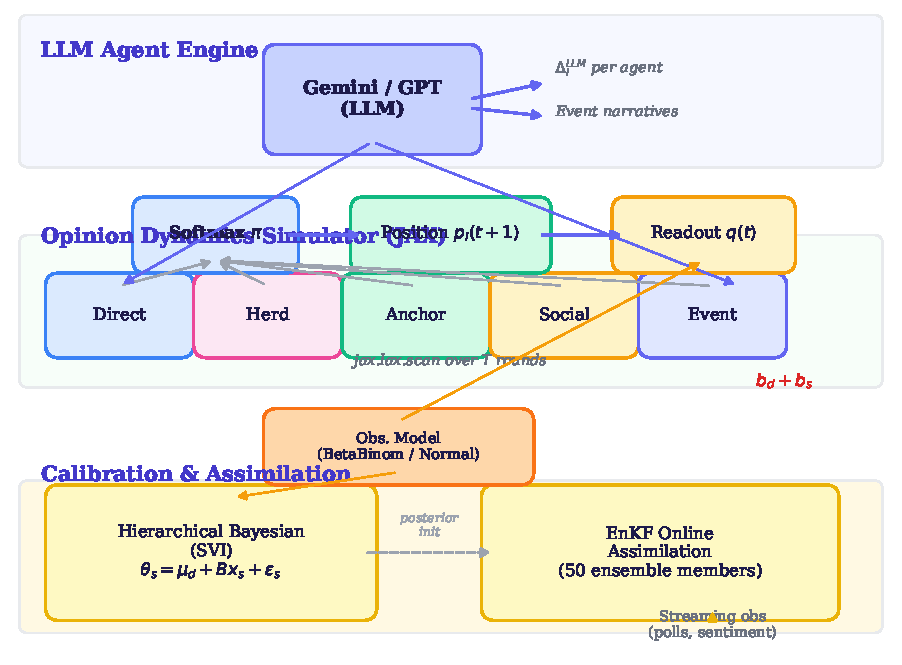
\includegraphics[width=\textwidth]{figures/fig1_architecture.pdf}
    \caption{System architecture diagram. Three horizontal layers. \textbf{Top layer} --- ``LLM Agent Engine'': Gemini/GPT producing $\Delta^{\text{LLM}}$ per agent and event narratives. \textbf{Middle layer} --- ``Opinion Dynamics Simulator (JAX)'': five force boxes (Direct, Herd, Anchor, Social, Event) feeding into softmax $\pi$, then position update $p(t+1)$, then readout $q(t)$, with \texttt{jax.lax.scan} over $T$ rounds. \textbf{Bottom layer} --- ``Calibration \& Assimilation'': hierarchical Bayesian (SVI) with observation model feeding upward to readout, and EnKF Online with bidirectional connection to streaming observations. Dashed arrow from SVI posterior to EnKF initialization. Annotations: $b_d + b_s$ on the readout-to-observation connection; $\theta_s = \mu_d + Bx_s + \varepsilon_s$ between hierarchy and simulator.}
    \label{fig:architecture}
\end{figure}

\subsection{Agent State Space}

Each agent $i \in \{1, \ldots, n\}$ maintains a scalar position $p_i(t) \in [-1, +1]$ representing their stance on a binary issue, where $+1$ denotes maximum support (``Pro'') and $-1$ maximum opposition (``Against''). Agents are characterized by three fixed attributes:

\begin{itemize}
    \item \textbf{Type} $\tau_i \in \{\text{elite}, \text{citizen}\}$: determines step size and behavioral parameters.
    \item \textbf{Rigidity} $\rho_i \in [0, 1]$: resistance to opinion change. Elites have higher rigidity ($\rho \approx 0.7$) than citizens ($\rho \approx 0.3$).
    \item \textbf{Tolerance} $\theta_i \in [0, 1]$: radius of the bounded-confidence window for social influence. Elites have lower tolerance ($\theta \approx 0.3$) than citizens ($\theta \approx 0.6$).
\end{itemize}

Agents interact through a sparse weighted graph $W \in \mathbb{R}^{n \times n}$ constructed from LLM-assigned influence scores using a $k$-nearest-neighbor scheme ($k = 5$, matching the NumPy simulation's feed-based top-5 selection).

\subsection{Five Force Terms}

At each round $t$, five independent forces act on each agent. The taxonomy draws on three established traditions: (i)~bounded-confidence models of social influence \citep{deffuant2000,hegselmann2002}, which motivate Forces 2 and 4 (herd behavior and social influence with tolerance gating); (ii)~anchoring and commitment theory \citep{festinger1957}, which motivates Force 3 (anchor rigidity with gradual drift); and (iii)~exogenous shock models from political science, which motivate Force 5 (event shock). Force 1 (direct LLM influence) is novel to the LLM-agent setting and has no classical analog. We do not claim completeness: the model omits mechanisms known to matter in specific domains---notably trust cascades in financial crises, institutional contagion, and information asymmetries (see Section~\ref{sec:discussion} for a systematic discussion of missing forces). The five forces are chosen as the minimal set that spans the dominant variance in our 42-scenario dataset, as confirmed by the Sobol analysis (Section~\ref{sec:sobol}), which shows that these forces account for $>85\%$ of total output variance. The forces capture distinct social mechanisms:

\textbf{Force 1: Direct LLM Influence.} The LLM generates per-agent opinion shifts $\Delta_i^{\text{LLM}}(t)$ based on the current narrative context. The direct force is:

\begin{equation}\label{eq:1}
f_i^{\text{direct}}(t) = \Delta_i^{\text{LLM}}(t) \cdot (1 - \rho_i) \cdot \max(0, 1 - |p_i(t)|)
\end{equation}

The susceptibility factor $(1 - \rho_i)$ attenuates influence on rigid agents, while the boundary factor $\max(0, 1 - |p_i|)$ prevents extreme agents from being pushed further.

\textbf{Force 2: Herd Behavior (Consensus Pull).} Agents experience a pull toward the weighted mean of their neighborhood when the deviation exceeds a learned threshold $\theta_h$:

\begin{equation}\label{eq:2}
f_i^{\text{herd}}(t) = (\bar{p}_i^{\text{feed}} - p_i) \cdot (1 - \rho_i) \cdot \sigma\!\left(\frac{|\bar{p}_i^{\text{feed}} - p_i| - \theta_h}{\tau_H}\right)
\end{equation}

where $\bar{p}_i^{\text{feed}}$ is the normalized weighted mean of neighbors' positions, $\theta_h = \sigma(\text{logit\_herd\_threshold})$ is a learned threshold, and $\tau_H = 0.02$ is a steepness parameter. The sigmoid activation creates a smooth transition: agents ignore small deviations but respond to large consensus gaps.

\textbf{Force 3: Anchor Rigidity.} A restorative force pulling agents toward their original position:

\begin{equation}\label{eq:3}
f_i^{\text{anchor}}(t) = \rho_i \cdot (p_i^{\text{orig}}(t) - p_i(t))
\end{equation}

where $p_i^{\text{orig}}(t)$ drifts slowly toward the current position at rate $\delta_{\text{drift}} = \sigma(\text{logit\_anchor\_drift})$, modeling gradual internalization of new positions.

\textbf{Force 4: Social Influence (Bounded Confidence).} Weighted averaging with tolerance-gated interaction:

\begin{equation}\label{eq:4}
f_i^{\text{social}}(t) = \frac{\sum_j w_{ij}(t) \cdot (p_j(t) - p_i(t))}{\sum_j w_{ij}(t) + \epsilon}
\end{equation}

where $w_{ij}(t) = W_{ij} \cdot \sigma\!\left(\frac{\theta_i - |p_j - p_i|}{\tau_{BC}}\right)$, $\tau_{BC} = 0.02$, and $\epsilon = 10^{-8}$. The $\epsilon$ prevents numerical instability when an agent's tolerance window excludes all neighbours (making $\sum_j w_{ij} \approx 0$); in this edge case the social force vanishes gracefully rather than producing undefined gradients. This implements smooth bounded confidence: agents preferentially interact with like-minded peers, but the transition is differentiable rather than a hard cutoff.

\textbf{Force 5: Exogenous Event Shock.} External events apply a uniform directional push:

\begin{equation}\label{eq:5}
f_i^{\text{event}}(t) = m_t \cdot d_t \cdot (1 - \rho_i)
\end{equation}

where $m_t \in [0, 1]$ is the event magnitude and $d_t \in \{-1, +1\}$ its direction. Events are generated by the LLM based on the simulated scenario narrative.

\subsection{Force Standardization}

Raw forces have heterogeneous scales (e.g., social forces depend on graph density, event forces on shock magnitude). We standardize all five forces per round using exponential moving averages:

\begin{equation}\label{eq:6}
\tilde{f}_k(t) = \frac{f_k(t) - \mu_k(t)}{\sigma_k(t) + \epsilon}
\end{equation}

where $\mu_k(t)$ and $\sigma_k(t)$ are updated via EMA with decay $\alpha = 0.3$, computed across all agents in each round. The per-round statistics are symmetric functions over the agent set, ensuring permutation invariance ($\max |\Delta\text{pro\_fraction}| < 6 \times 10^{-8}$ under random agent permutation).

\textbf{Trade-off.} Subtracting the cross-sectional mean preserves \emph{relative} susceptibility differences across agents but attenuates the common directional component of forces that act uniformly---most notably event shocks (Force~5) and direct LLM influence (Force~1), which push all agents in the same direction. The softmax mixing then operates on the agent-specific \emph{deviations} from the population mean rather than on the absolute force magnitudes. This design choice prioritises scale normalisation and gradient stability over preservation of macro-directional signals. In practice, the attenuated common component is partially recovered by the learnable force weights $\alpha_k$, which can amplify the standardised residuals. Nevertheless, the standardisation may cause the calibration to underestimate the influence of uniformly directional forces relative to heterogeneous forces like social influence. We discuss this further as a methodological limitation in Section~\ref{sec:discussion}.

\subsection{Gauge-Fixed Softmax Mixing}

The five standardized forces are combined through a softmax mixture with a gauge-fixing constraint:

\begin{equation}\label{eq:7}
\boldsymbol{\alpha} = [0, \alpha_h, \alpha_a, \alpha_s, \alpha_e]^\top
\end{equation}

\begin{equation}\label{eq:8}
\pi_k = \text{softmax}(\boldsymbol{\alpha})_k, \quad \sum_k \pi_k = 1
\end{equation}

The direct force weight $\alpha_{\text{direct}} \equiv 0$ serves as the reference level (gauge), resolving the shift invariance of softmax. This means the four remaining weights $\alpha_h, \alpha_a, \alpha_s, \alpha_e$ are interpretable as log-odds relative to the direct LLM influence.

The combined force per agent is:

\begin{equation}\label{eq:9}
\tilde{f}_i^{\text{combined}}(t) = \sum_k \pi_k \cdot \tilde{f}_{k,i}(t)
\end{equation}

\subsection{Position Update}

The position update applies a type-specific step size with smooth clamping:

\begin{equation}\label{eq:10}
\Delta p_i = \lambda_{\tau_i} \cdot \tilde{f}_i^{\text{combined}}, \quad \Delta p_i^{\text{clamped}} = \tanh\!\left(\frac{\Delta p_i}{c_{\tau_i}}\right) \cdot c_{\tau_i}
\end{equation}

where $\lambda_{\text{elite}} = \exp(\log \lambda_{\text{elite}})$, $\lambda_{\text{citizen}} = \exp(\log \lambda_{\text{citizen}})$, $c_{\text{elite}} = 0.15$, $c_{\text{citizen}} = 0.25$. The $\tanh$ clamping provides smooth saturation rather than hard clipping, preserving differentiability.

The final update is:

\begin{equation}\label{eq:11}
p_i(t+1) = \text{clip}(p_i(t) + \Delta p_i^{\text{clamped}}, -1, +1)
\end{equation}

\subsection{Readout Function}

The mapping from agent positions to aggregate opinion uses a soft classification:

\begin{equation}\label{eq:12}
\text{pro}(t) = \frac{\sum_i \sigma\!\left(\frac{p_i(t) - 0.05}{0.02}\right)}{\sum_i \left[\sigma\!\left(\frac{p_i(t) - 0.05}{0.02}\right) + \sigma\!\left(\frac{-p_i(t) - 0.05}{0.02}\right)\right]}
\end{equation}

This readout excludes near-neutral agents ($|p_i| < 0.05$) from the decided count, producing $\text{pro\_fraction} \in [0, 1]$. The 0.02 temperature ensures smooth but sharp classification.

\subsection{Parameter Summary}

The model has 8 mechanistic parameters, partitioned into 4 calibrable and 4 frozen:

\begin{table}[H]
\centering
\caption{Model Parameters}
\label{tab:params}
\begin{adjustbox}{max width=\textwidth}
\begin{tabular}{@{}llp{5.5cm}ll@{}}
\toprule
Parameter & Symbol & Role & Type & Default \\
\midrule
Herd weight & $\alpha_h$ & Consensus pull strength (log-odds vs direct) & Calibrable & --- \\
Anchor weight & $\alpha_a$ & Rigidity pull strength & Calibrable & --- \\
Social weight & $\alpha_s$ & Bounded-confidence averaging strength & Calibrable & --- \\
Event weight & $\alpha_e$ & Exogenous shock strength & Calibrable & --- \\
Elite step & $\log \lambda_{\text{elite}}$ & Step magnitude for elite agents & Frozen & $-1.2$ \\
Citizen step & $\log \lambda_{\text{citizen}}$ & Step magnitude for citizen agents & Frozen & $-0.5$ \\
Herd threshold & $\text{logit}\;\theta_h$ & Min.\ deviation to trigger herd & Frozen & $0.5$ \\
Anchor drift & $\text{logit}\;\delta_{\text{drift}}$ & Rate of anchor position drift & Frozen & $-1.4$ \\
\bottomrule
\end{tabular}
\end{adjustbox}
\end{table}

The calibrable/frozen partition is a pragmatic choice informed by Sobol sensitivity analysis (Section~\ref{sec:sobol}), which identifies the four calibrable parameters as the most influential; however, at least one frozen parameter ($\lambda_{\text{citizen}}$, $S_T = 0.121$) remains non-negligible (Section~\ref{sec:discussion}).

\subsection{LLM Agent Engine}
\label{sec:llm_methodology}

The LLM provides two inputs to the force system: per-agent opinion shifts $\Delta_i^{\text{LLM}}(t)$ (Force~1) and event narratives with magnitude $m_t$ and direction $d_t$ (Force~5). Both are generated by Google Gemini (\texttt{gemini-2.0-flash-lite}), a lightweight model selected for cost efficiency across 42 multi-round scenarios.

\textbf{Prompting.} Each round, the LLM receives a structured prompt containing: the scenario description, current agent positions and attributes, the social graph neighbourhood, recent events, and the current narrative context. The prompt requests a JSON response with a numerical opinion shift $\Delta \in [-1, +1]$, a brief reasoning chain, and optional coalition/sentiment metadata. Events are generated separately via a scenario-context prompt that requests magnitude, direction, and narrative description. All prompts use zero-shot instruction following (no few-shot examples). Full prompt templates are available in the code repository.

\textbf{Temperature and sampling.} All LLM calls use temperature $T = 0.7$ with top-$p = 0.95$. Each scenario is run once (single seed) per calibration version; the resulting $\Delta^{\text{LLM}}$ values and events are cached and reused across all SVI optimization steps to ensure deterministic gradients.

\textbf{Inter-run variance.} Because each scenario uses a single LLM rollout, inter-run variance is not measured directly. The discrepancy terms $b_d$ and $b_s$ absorb both structural model error and LLM stochasticity without separating the two. Running multiple LLM rollouts per scenario (e.g., 5--10 seeds) would enable decomposing discrepancy into LLM variance vs.\ opinion-dynamics misspecification; we identify this as a high priority for future work (Section~\ref{sec:discussion}).

\textbf{Reproducibility caveat.} LLM outputs are not bitwise reproducible across API versions. The $\Delta^{\text{LLM}}$ values used in this paper were generated in January 2026; reproducing the exact numerical results requires the cached outputs (included in the repository).

\section{Hierarchical Bayesian Calibration}
\label{sec:calibration}

\subsection{Motivation}

A single set of global parameters cannot adequately describe opinion dynamics across diverse domains. Political referenda involve different social mechanisms than corporate crises or public health debates. At the same time, per-scenario calibration with 4 parameters and limited per-scenario data (typically 3--9 polling observations) leads to severe overfitting. A hierarchical model enables partial pooling: scenarios share information through domain and global priors while retaining scenario-specific flexibility through model discrepancy terms.

\subsection{Three-Level Hierarchy}

The model has three levels:

\textbf{Level 1 (Global).} Shared priors on the mixing weights:

\begin{equation}\label{eq:13}
\mu_{\text{global}} \sim \mathcal{N}(\mathbf{0}, I_4), \quad \sigma_{\text{global}} \sim \text{HalfNormal}(0.3)
\end{equation}

where $\mu_{\text{global}} \in \mathbb{R}^4$ represents the global mean of the four calibrable alpha parameters.

\textbf{Level 2 (Domain).} Each domain $d \in \{\text{political}, \text{financial}, \text{corporate}, \ldots\}$ has domain-level parameter means:

\begin{equation}\label{eq:14}
\mu_d \sim \mathcal{N}(\mu_{\text{global}}, \text{diag}(\sigma_{\text{global}}^2))
\end{equation}

where $\mu_d \in \mathbb{R}^4$ are the domain-level alpha parameters.

\textbf{Domain-level identifiability caveat.} Of the 10 domains, only 3 have $N \geq 4$ training scenarios (political: 11, corporate: 6, financial: 6); 5 domains have $N \leq 2$ (energy, labor, commercial, environmental, social). For these under-represented domains, the domain-level parameters $\mu_d$ are effectively determined by the global prior rather than by within-domain data, and the domain-level discrepancy $b_d$ is unidentifiable from the scenario-level $b_s$. We retain the 10-domain hierarchy because it is the correct generative structure (domains \emph{do} differ mechanistically), but readers should interpret domain-level estimates for $N \leq 2$ domains as prior-dominated rather than data-driven. Table~\ref{tab:domain_discrepancy} marks these with $\ddagger$.

\textbf{Level 3 (Scenario).} Each scenario $s$ has scenario-specific parameters drawn from its domain:

\begin{equation}\label{eq:15}
\theta_s \sim \mathcal{N}(\mu_{d(s)} + B \cdot x_s, \text{diag}(\sigma_d^2))
\end{equation}

where $\theta_s \in \mathbb{R}^4$ are the four softmax weights used for simulation, $\sigma_d \in \mathbb{R}^4$ is a domain-specific dispersion (not the global $\sigma_{\text{global}}$), and $B \cdot x_s$ is the covariate regression defined in Section~\ref{sec:covariates}. The domain-level variance $\sigma_d$ allows different domains to have different degrees of scenario-to-scenario heterogeneity.

\subsection{Readout Discrepancy}

The simulator is structurally misspecified: LLM-generated narratives cannot perfectly reproduce real-world opinion formation. Rather than absorbing this misspecification into the parameters (which would bias them), we model it explicitly through additive correction in logit space on the readout.

The discrepancy operates on the scalar readout ($\mathbb{R}^1$), not on the parameter space ($\mathbb{R}^4$):

\begin{equation}\label{eq:16}
b_d \sim \mathcal{N}(0, \sigma_{b,\text{between}}^2), \quad \sigma_{b,\text{between}} \sim \text{HalfNormal}(0.2)
\end{equation}

\begin{equation}\label{eq:17}
b_s \sim \mathcal{N}(0, \sigma_{b,\text{within}}^2), \quad \sigma_{b,\text{within}} \sim \text{HalfNormal}(0.5)
\end{equation}

where $b_d \in \mathbb{R}$ is the domain-level readout bias (between-domain discrepancy) and $b_s \in \mathbb{R}$ is the scenario-specific readout discrepancy (within-domain). The corrected readout for scenario $s$ in domain $d$ is:

\begin{equation}\label{eq:18}
q_s^{\text{corrected}} = \sigma\!\left(\text{logit}(q_s^{\text{sim}}) + b_d + b_s\right)
\end{equation}

where $q_s^{\text{sim}}$ is the raw simulator output. By operating in logit space, the correction is unbounded and additive while the sigmoid guarantees the result remains in $[0, 1]$. This decomposition follows \citet{kennedy2001}: the calibrated parameters $\theta$ represent genuine opinion dynamics mechanisms, while the discrepancy terms $b_d$ and $b_s$ absorb systematic simulator errors.

\subsection{Observation Model}

For scenarios with per-round polling data (sample size $n_t$, observed count $y_t$):

\begin{equation}\label{eq:19}
y_t \mid q_t, \phi \sim \text{BetaBinomial}(n_t, q_t \cdot \phi, (1 - q_t) \cdot \phi)
\end{equation}

where $\phi = \exp(\log \phi)$ is a learned concentration parameter. The BetaBinomial accounts for both sampling noise (binomial) and overdispersion (beta mixing).

For scenarios with only a final outcome:

\begin{equation}\label{eq:20}
y_{\text{final}} \mid q_T, \sigma_{\text{obs}} \sim \mathcal{N}(100 \cdot q_T, \sigma_{\text{obs}}^2)
\end{equation}

where $\sigma_{\text{obs}} = \exp(\log \sigma)$ is learned.

\subsection{Inference via SVI}

The posterior is intractable due to the nonlinear JAX simulator in the likelihood. We use stochastic variational inference (SVI) with an AutoLowRankMultivariateNormal guide in NumPyro, which approximates the posterior with a low-rank plus diagonal covariance structure:

\begin{equation}\label{eq:21}
q(\theta) = \mathcal{N}(\mu_q, D + VV^\top)
\end{equation}

where $D$ is diagonal and $V$ has rank $\leq \dim(\theta)$. This captures dominant posterior correlations (e.g., between $\alpha_h$ and $\alpha_a$) while scaling to the full parameter space.

The SVI objective is the evidence lower bound (ELBO):

\begin{equation}\label{eq:22}
\mathcal{L}(\mu_q, D, V) = \mathbb{E}_{q(\theta)}[\log p(y \mid \theta) + \log p(\theta)] - \mathbb{E}_{q(\theta)}[\log q(\theta)]
\end{equation}

minimized over 3000 steps with learning rate 0.002 and cosine annealing. Gradients are computed via JAX automatic differentiation through the full simulate $\to$ readout $\to$ likelihood chain.

\textbf{Important caveat on uncertainty estimates.} A comparison with gold-standard NUTS (Section~\ref{sec:svi_nuts}) reveals that the SVI posterior agrees with NUTS on dominant parameters ($\alpha_{\text{herd}}$: $|\Delta\mu|/\sigma_{\text{NUTS}} = 0.15$; $\alpha_{\text{anchor}}$: 0.35) but substantially underestimates uncertainty on weaker ones ($\alpha_{\text{social}}$: 0.85; $\alpha_{\text{event}}$: 1.71), with SVI standard deviations 5--13$\times$ narrower. This means that all credible intervals reported in this paper are likely too narrow for $\alpha_{\text{social}}$ and $\alpha_{\text{event}}$. The effect on coverage is not identifiable from this comparison alone: wider NUTS intervals could raise or lower coverage depending on whether the shifted posterior means move intervals toward or away from ground truth. Without a full NUTS calibration on all 42 scenarios, the reported 75.0\% test coverage (\textsc{Base}) cannot be directly compared to what exact inference would yield. This limitation pervades all downstream uncertainty estimates, including the coverage figures across variants and the EnKF ensemble spread.

\subsection{Covariate Regression}
\label{sec:covariates}

The covariate regression is incorporated directly into the scenario-level prior (\eqref{eq:15}, Section~4.2). The matrix $B \in \mathbb{R}^{4 \times 5}$ and covariates $x_s \in \mathbb{R}^5$ are defined as follows:

\begin{enumerate}
    \item \textbf{initial\_polarization} --- initial spread of agent positions
    \item \textbf{event\_volatility} --- intensity and frequency of external shocks
    \item \textbf{elite\_concentration} --- power centralization among top agents
    \item \textbf{institutional\_trust} --- public confidence in institutions (0--1)
    \item \textbf{undecided\_share} --- initial proportion of near-neutral agents
\end{enumerate}

The prior on $B$ is informative but weakly regularizing: $B_{ij} \sim \mathcal{N}(0, 0.3)$, allowing the data to determine whether covariates have predictive power. A covariate effect is considered significant if its 95\% CI excludes zero.

\section{Calibration Results}
\label{sec:results}

\subsection{Dataset}

We curated 42 empirical scenarios across 10 domains, each with a ground-truth final outcome and, where available, intermediate polling data. The scenarios span 2012--2023 and cover political referenda, financial crises, corporate controversies, public health debates, technology policy, and social movements.

\begin{table}[H]
\centering
\caption{Dataset Composition by Domain}
\label{tab:dataset}
\begin{tabular}{llll}
\toprule
Domain & N (Train) & N (Test) & Example Scenarios \\
\midrule
Political & 11 & 3 & Brexit, Scottish Independence, Chilean Constitution \\
Corporate & 6 & 1 & Dieselgate, Boeing 737 MAX, Facebook$\to$Meta \\
Financial & 6 & 1 & FTX collapse, GameStop squeeze, SVB collapse \\
Public Health & 4 & 1 & COVID vaccination (IT), AstraZeneca controversy \\
Technology & 2 & 1 & Net Neutrality repeal \\
Commercial & 1 & 1 & Tesla Cybertruck reveal \\
Energy & 1 & 0 & Japanese nuclear phase-out \\
Environmental & 1 & 0 & Keystone XL pipeline \\
Labor & 1 & 0 & Uber vs.\ taxi regulation \\
Social & 1 & 0 & Marriage equality \\
\midrule
\textbf{Total} & \textbf{34} & \textbf{8} & \\
\bottomrule
\end{tabular}
\end{table}

The train/test split is stratified by domain with approximately 80/20 ratio.

Scenarios flagged as \texttt{NEEDS\_VERIFICATION} during the review phase (prior to calibration) are reported separately in a pre-specified sensitivity analysis. This flag is assigned based on data quality criteria---missing primary sources, interpolated polling without verification, data-quality-flagged ground-truth encoding---not based on model performance. One test scenario (Archegos Capital Collapse, quality\_score = 67 on a 0--100 scale where $<70$ triggers the flag) carries this label. The canonical test metrics use the full $N=8$ test set including flagged scenarios; verified-only ($N=7$) results are reported alongside as sensitivity analysis throughout.

\subsection{Calibrated Global Parameters}

SVI converges in 3000 steps (final ELBO loss: 514.7) with a total runtime of 40.2 minutes for Phase B (empirical fine-tuning) and 0.4 minutes for Phase C (validation).

\begin{table}[H]
\centering
\caption{Calibrated Global Posterior}
\label{tab:global_posterior}
\begin{adjustbox}{max width=\textwidth}
\begin{tabular}{@{}llll@{}}
\toprule
Parameter & Mean & 95\% CI & Interpretation \\
\midrule
$\alpha_{\text{herd}}$ & $-0.176$ & $[-0.265, -0.079]$ & Herd below direct influence \\
$\alpha_{\text{anchor}}$ & $+0.297$ & $[+0.199, +0.401]$ & Anchor rigidity strongest \\
$\alpha_{\text{social}}$ & $-0.105$ & $[-0.202, -0.005]$ & Social influence below direct \\
$\alpha_{\text{event}}$ & $-0.130$ & $[-0.227, -0.033]$ & Event shocks below direct \\
$\sigma_{\text{global}}$ & $[0.135, 0.147, 0.144, 0.143]$ & --- & Inter-scenario spread \\
\bottomrule
\end{tabular}
\end{adjustbox}
\end{table}

The positive $\alpha_{\text{anchor}}$ indicates that anchor rigidity (resistance to change) dominates the force mixture. This is consistent with the well-documented status quo bias in opinion dynamics: people tend to revert toward their initial positions after temporary shifts. The negative values for $\alpha_{\text{herd}}$, $\alpha_{\text{social}}$, and $\alpha_{\text{event}}$ indicate these forces are present but weaker than direct LLM influence (the gauge reference).

Converting to softmax weights: $\pi = \text{softmax}([0, -0.176, 0.297, -0.105, -0.130]) \approx [0.201, 0.169, 0.271, 0.181, 0.177]$. Anchor rigidity receives approximately 27.1\% of the total weight, direct influence 20.1\%, social conformity 18.1\%, event shocks 17.7\%, and herd behavior 16.9\%.

\subsection{Readout Discrepancy}

The calibrated discrepancy parameters reveal the scale of structural model misspecification:

\begin{equation}\label{eq:23}
\sigma_{b,\text{between}} = 0.115 \quad [0.073, 0.173]
\end{equation}
\begin{equation}\label{eq:24}
\sigma_{b,\text{within}} = 0.558 \quad [0.436, 0.696]
\end{equation}

The within-scenario discrepancy ($\sigma_{b,\text{within}} = 0.558$) is approximately 5$\times$ the between-domain discrepancy ($\sigma_{b,\text{between}} = 0.115$), indicating that scenario-specific factors dominate over systematic domain-level biases. In practical terms, 0.558 in logit space translates to approximately 12--14 percentage points of systematic prediction error that the model cannot eliminate through parameter adjustment alone.

\begin{table}[H]
\centering
\caption{Domain-Level Readout Discrepancy. Only domains with $N \geq 3$ training scenarios are shown individually; the remaining 6 domains (commercial, energy, environmental, labor, social, technology; $N \leq 2$ each, 7 training scenarios total) are collapsed into ``Other'' because the hierarchical model cannot produce reliable domain-level estimates at those sample sizes.}
\label{tab:domain_discrepancy}
\begin{adjustbox}{max width=\textwidth}
\begin{tabular}{@{}llllll@{}}
\toprule
Domain & N & $b_d$ Mean & 95\% CI & Mean $|b_s|$ & Bias \\
\midrule
Financial     & 6  & $-0.054$ & $[-0.242, +0.126]$ & 0.744 & Over-predicts \\
Corporate     & 6  & $-0.040$ & $[-0.221, +0.139]$ & 0.432 & Over-predicts \\
Public Health & 4  & $-0.032$ & $[-0.223, +0.164]$ & 0.534 & Over-predicts \\
Political     & 11 & $+0.019$ & $[-0.145, +0.183]$ & 0.198 & No systematic bias \\
\midrule
Other ($N \leq 2$) & 7 & $-0.007$ & --- & 0.268 & Pooled; no domain-level inference \\
\bottomrule
\end{tabular}
\end{adjustbox}
\end{table}

Financial scenarios exhibit the largest mean absolute discrepancy ($|b_s| = 0.744$), driven by cases where the model systematically over-predicts support levels. The political domain, with the most training data ($N = 11$), shows the lowest systematic bias ($b_d \approx 0$, mean $|b_s| = 0.198$). Six domains with $N \leq 2$ training scenarios each are collapsed because single-scenario domain-level estimates are determined almost entirely by the global prior rather than the data; reporting them individually would convey more structural insight than the data support.

\subsection{Predictive Performance}

Credible intervals are computed in logit space and back-transformed via sigmoid, guaranteeing $[0, 100]$ bounds by construction.

\begin{table}[H]
\centering
\caption{Validation Metrics (Test Set)}
\label{tab:validation_metrics}
\begin{tabular}{lll}
\toprule
Metric & Full Test ($N=8$) & Verified Only ($N=7$) \\
\midrule
MAE & 19.2~pp & 12.6~pp \\
RMSE & 26.6 & 14.3 \\
Median AE & 11.9~pp & 9.2~pp \\
Coverage 90\% & 75.0\% & 85.7\% \\
Coverage 50\% & 37.5\% & 42.9\% \\
CRPS & 15.4 & 8.6 \\
\bottomrule
\end{tabular}
\end{table}

The canonical metric is the full-test MAE of 19.2~pp ($N = 8$), with test-set coverage of 75.0\% (6/8 scenarios within 90\% CI; Clopper--Pearson 95\% binomial CI: [34.9\%, 96.8\%]). The wide binomial CI reflects the fundamental limitation of evaluating coverage on $N = 8$: a single scenario flipping changes coverage by 12.5~pp. As a pre-specified sensitivity analysis, excluding Archegos (flagged \texttt{NEEDS\_VERIFICATION}, error = 65.0~pp) yields 12.6~pp MAE and 85.7\% coverage on $N = 7$ (binomial CI: [42.1\%, 99.6\%]). This illustrates both the outsized influence of a single financial outlier and the imprecision of small-sample coverage estimates.

\begin{table}[H]
\centering
\caption{Test Set Detailed Results}
\label{tab:test_detailed}
\begin{adjustbox}{max width=\textwidth}
\begin{tabular}{@{}lllllll@{}}
\toprule
Scenario & Domain & GT (\%) & Predicted $\mu \pm \sigma$ & Error (pp) & 90\% CI & Covered \\
\midrule
Archegos Capital*$^\dagger$ & Financial & 35.0 & $>$99\%$^{\ddagger}$ & +65.0 & [98.5, 100.0] & \texttimes \\
Greek Bailout & Political & 38.7 & 65.3 $\pm$ 11.7 & +26.6 & [42.7, 84.5] & \texttimes \\
Net Neutrality & Technology & 83.0 & 66.3 $\pm$ 12.6 & $-$16.7 & [47.3, 82.8] & \checkmark \\
French Election & Political & 66.1 & 51.6 $\pm$ 13.7 & $-$14.5 & [29.7, 72.8] & \checkmark \\
COVID Vax (IT) & Pub.\ Health & 80.0 & 70.8 $\pm$ 11.2 & $-$9.2 & [52.1, 88.7] & \checkmark \\
Tesla Cybertruck & Commercial & 62.0 & 54.1 $\pm$ 14.7 & $-$7.9 & [26.1, 72.6] & \checkmark \\
Amazon HQ2 & Corporate & 56.0 & 63.3 $\pm$ 12.9 & +7.3 & [48.7, 80.6] & \checkmark \\
Turkish Ref. & Political & 51.4 & 57.5 $\pm$ 13.0 & +6.1 & [37.4, 75.7] & \checkmark \\
\bottomrule
\end{tabular}
\end{adjustbox}

\vspace{4pt}
\footnotesize
*\texttt{NEEDS\_VERIFICATION} --- flagged prior to calibration; included in canonical full-test metrics, reported separately in verified-only sensitivity analysis. CI computed in logit space and back-transformed.

$^\dagger$ The Archegos 65~pp error reflects fundamental model misspecification: the simulator's LLM-generated trajectory produces a consensus narrative that saturates the sigmoid readout (predicted $>$99\% support vs.\ GT 35\%). This is a genuine prediction failure, not a numerical artifact.

$^\ddagger$ Archegos posterior is in the sigmoid saturation region; logit-space CI $[3.8, 5.4]$ maps to $[97.8, 99.6]\%$ after back-transformation. The reported mean and CI are approximate due to numerical precision at sigmoid extremes.
\end{table}

\subsection{Worst-Case Scenarios}

\begin{table}[H]
\centering
\caption{Top 5 Scenario Discrepancies (Training Set)}
\label{tab:worst_case}
\begin{tabular}{lllll}
\toprule
Scenario & Domain & $b_s$ & Error (pp) & Failure Mode \\
\midrule
WeWork IPO & Financial & $-1.378$ & +48.5 & Trust collapse not modeled \\
United Airlines & Corporate & $-0.860$ & +15.4 & Viral outrage underestimated \\
SVB Collapse & Financial & $-0.835$ & +38.1 & Sequential shocks mishandled \\
Chile Constitution & Political & $+0.816$ & $-$41.5 & Landslide momentum missing \\
FTX Crypto & Financial & $-0.727$ & +11.0 & Contagion dynamics absent \\
\bottomrule
\end{tabular}
\end{table}

The three largest discrepancies are all financial crises where the model over-predicts support (negative $b_s$). This systematic failure motivates the regime-switching extension developed in Section~\ref{sec:regime}.

The \textsc{Base} calibration represents a substantial methodological advance over the earlier v1 prototype, which used grid search on synthetic scenarios without uncertainty quantification or model discrepancy. A detailed comparison is provided in Appendix~\ref{app:supplementary} (Table~\ref{tab:v1v2}).

Exploratory covariate analysis of the domain-level regression matrix $B$ yields one nominally significant effect ($\alpha_{\text{event}} \times \text{institutional\_trust}$: higher trust reduces event sensitivity). However, with 20 regression coefficients estimated from $N=34$ scenarios, this result should be interpreted with caution: a Bonferroni-corrected threshold ($\alpha/20 = 0.0025$) would render it non-significant. We report it as hypothesis-generating rather than confirmatory. Full results are in Appendix~\ref{app:supplementary}.

\section{Calibration Variants}
\label{sec:evolution}

The \textsc{Base} calibration on 42 scenarios (34 train / 8 test) is the \textbf{main result} of this paper. All primary claims---posterior estimates, coverage, Sobol analysis, SBC validation---rest on \textsc{Base}. Three exploratory variants were investigated as sensitivity analyses; because they use different datasets, splits, and---for \textsc{Poll}---additional information (polling data), they are \emph{not directly comparable} to \textsc{Base} or to each other. Detailed descriptions are in Appendix~\ref{app:evolution_details}; we summarise the key findings here.

Each variant targets a specific hypothesis about the dominant error source. Table~\ref{tab:variant_names} defines the naming convention used throughout.

\begin{table}[H]
\centering
\caption{Calibration variant names and key design choices.}
\label{tab:variant_names}
\begin{adjustbox}{max width=\textwidth}
\begin{tabular}{@{}lllll@{}}
\toprule
Name & Events & Dataset & Polling & Design hypothesis \\
\midrule
\textsc{Base} & LLM-generated & 42 (34/8) & Not used & Discrepancy model absorbs LLM error \\
\textsc{Ground} & Verified (high-$|b_s|$ domains) & 42 (34/8) & Not used & Verified events reduce domain bias \\
\textsc{Hybrid} & LLM agents + verified events & 20 (15/5) & Not used & Curated data + hybrid events improve accuracy \\
\textsc{Poll}$^\dagger$ & LLM agents + verified events & 20 (15/5) & Initial poll & Poll anchor corrects LLM centrist bias \\
\bottomrule
\multicolumn{5}{@{}l}{\footnotesize $^\dagger$Uses strictly more information than other variants (initial polling observation).}
\end{tabular}
\end{adjustbox}
\end{table}

\textbf{\textsc{Ground}} replaced LLM events with verified events in high-discrepancy domains but collapsed training coverage from 79.4\% to 2.9\%, demonstrating that the discrepancy budget is load-bearing: when LLM-generated events are removed, the model loses the flexibility to absorb misspecification. \textbf{\textsc{Hybrid}} achieved 11.4~pp test MAE on a curated 20-scenario subset, but with a smaller test set ($N=5$ vs.\ 8), making direct comparison with \textsc{Base} impossible. \textbf{\textsc{Poll}} added a poll-informed anchor agent whose initial position reflects the empirical opinion distribution, improving training coverage to 86.7\%; since it uses strictly more information, gains cannot be attributed to architecture alone. Test-set coverage is 80.0\% (4/5) for both \textsc{Hybrid} and \textsc{Poll}. Full metrics are in Table~\ref{tab:versions}.

No variant dominates on all metrics. The small, non-overlapping test sets prevent definitive ranking; these variants should be read as evidence that event quality, dataset curation, and auxiliary information each affect different aspects of calibration quality.

\section{Validation}
\label{sec:validation}

\subsection{Simulation-Based Calibration}

Simulation-based calibration (SBC; \citealp{talts2018}) verifies that the inference procedure recovers known parameters. We generate 100 synthetic datasets from the prior, run NUTS inference (200 warmup + 200 samples) on each, and test whether the posterior rank statistics are uniformly distributed.

\begin{table}[H]
\centering
\caption{SBC Results}
\label{tab:sbc}
\begin{tabular}{lllll}
\toprule
Parameter & N & KS Statistic & $p$-value & Verdict \\
\midrule
$\alpha_{\text{herd}}$ & 100 & 0.070 & 0.685 & PASS \\
$\alpha_{\text{anchor}}$ & 100 & 0.095 & 0.308 & PASS \\
$\alpha_{\text{social}}$ & 100 & 0.075 & 0.600 & PASS \\
$\alpha_{\text{event}}$ & 100 & 0.075 & 0.600 & PASS \\
$\tau_{\text{readout}}$ & 100 & 0.095 & 0.308 & PASS \\
$\sigma_{\text{obs}}$ & 100 & 0.105 & 0.205 & PASS \\
\bottomrule
\end{tabular}
\end{table}

SBC confirms that the generative model is well-specified and that a gold-standard NUTS backend recovers correct posteriors: all 6 parameters pass the KS uniformity test ($p > 0.20$). Rank histograms are shown in Appendix~\ref{app:supplementary} (Figure~\ref{fig:sbc}). However, SBC does not validate the SVI approximation used for the full empirical model, since SBC runs use NUTS.

The SBC configuration uses 10 agents and 7 rounds per synthetic scenario with $\text{Normal}(0, 0.3)$ priors. Total runtime: 297.6 seconds (approximately 3 seconds per instance).

\subsection{SVI vs NUTS Comparison}
\label{sec:svi_nuts}

To assess variational approximation quality, we compare SVI and NUTS posteriors on a 4-scenario subset spanning two domains.

\begin{table}[H]
\centering
\caption{SVI vs NUTS Posterior Comparison (4-scenario subset)}
\label{tab:svi_nuts}
\begin{adjustbox}{max width=\textwidth}
\begin{tabular}{@{}lllcc@{}}
\toprule
Parameter & SVI ($\mu \pm \sigma$) & NUTS ($\mu \pm \sigma$) & $|\Delta\mu|/\sigma_{\text{NUTS}}$ & Compat. \\
\midrule
$\alpha_{\text{herd}}$ & $-0.500 \pm 0.085$ & $-0.383 \pm 0.796$ & 0.148 & Yes \\
$\alpha_{\text{anchor}}$ & $+0.905 \pm 0.065$ & $+0.604 \pm 0.856$ & 0.352 & Yes \\
$\alpha_{\text{social}}$ & $-0.997 \pm 0.105$ & $-0.350 \pm 0.763$ & 0.848 & No \\
$\alpha_{\text{event}}$ & $-1.752 \pm 0.073$ & $-0.137 \pm 0.946$ & 1.707 & No \\
\bottomrule
\end{tabular}
\end{adjustbox}

\vspace{4pt}
\footnotesize
SVI: 1000 steps, Adam(lr = 0.01), AutoLowRankMVN guide. NUTS: 200 warmup + 200 samples, max\_tree\_depth = 8.
\end{table}

The two dominant parameters show good agreement ($\alpha_{\text{herd}}$: $|\Delta\mu|/\sigma_{\text{NUTS}} = 0.15$; $\alpha_{\text{anchor}}$: 0.35). The weaker parameters show larger divergence ($\alpha_{\text{social}}$: 0.85; $\alpha_{\text{event}}$: 1.71), consistent with the known tendency of structured variational families with restricted covariance to concentrate posterior mass. The SVI standard deviations are 5--13$\times$ narrower than the NUTS estimates, indicating that the variational approximation substantially underestimates posterior uncertainty on the less-constrained parameters.

\textbf{This is one of the central findings of the paper}, not a side caveat: because the reported credible intervals, test-set coverage, and downstream EnKF initialization all flow from the SVI posterior, the concentration bias propagates into every uncertainty estimate we report. The model is well-specified (SBC confirms this under NUTS), but the \emph{production} uncertainty is approximate. Concretely:

\begin{itemize}
    \item The posterior \emph{means} for the dominant parameters ($\alpha_{\text{herd}}$, $\alpha_{\text{anchor}}$) are reliably estimated by SVI; point predictions are therefore trustworthy.
    \item The posterior \emph{widths} on $\alpha_{\text{social}}$ and $\alpha_{\text{event}}$ are substantially underestimated. The effect on test-set coverage is ambiguous: wider NUTS intervals could increase coverage (more scenarios captured) or decrease it (if the shifted means move intervals away from ground truth). The reported 75.0\% test-set coverage under SVI is therefore neither an upper nor a lower bound on coverage under exact inference---it is simply not comparable without a full NUTS calibration on all 42 scenarios.
    \item Conservative users should apply post-hoc inflation of the variational posterior or run short NUTS chains initialized from the SVI optimum. We list this as a high-priority item in future work (\S\ref{sec:discussion}).
\end{itemize}

This comparison uses a 4-scenario subset for computational tractability; a full 42-scenario NUTS run would strengthen the comparison but requires substantially more compute.

\subsection{Global Sensitivity Analysis}
\label{sec:sobol}

Variance-based global sensitivity analysis \citep{sobol2001} decomposes output variance into contributions from individual parameters and their interactions. We evaluate all 8 model parameters using $N = 1024$ Saltelli samples (18,432 total simulator evaluations, $n = 30$ agents, 7 rounds).

\begin{table}[H]
\centering
\caption{Sobol Sensitivity Indices}
\label{tab:sobol}
\begin{tabular}{llll}
\toprule
Parameter & $S_1$ (Main Effect) & $S_T$ (Total Effect) & Type \\
\midrule
$\alpha_{\text{herd}}$ & $0.364 \pm 0.059$ & $0.555 \pm 0.055$ & Calibrable \\
$\alpha_{\text{anchor}}$ & $0.207 \pm 0.060$ & $0.452 \pm 0.047$ & Calibrable \\
$\alpha_{\text{social}}$ & $0.086 \pm 0.040$ & $0.213 \pm 0.034$ & Calibrable \\
$\alpha_{\text{event}}$ & $0.026 \pm 0.033$ & $0.115 \pm 0.023$ & Calibrable \\
$\lambda_{\text{citizen}}$ & $0.002 \pm 0.033$ & $0.121 \pm 0.025$ & Frozen \\
$\lambda_{\text{elite}}$ & $0.007 \pm 0.010$ & $0.016 \pm 0.006$ & Frozen \\
$\theta_{\text{herd}}$ & $0.003 \pm 0.013$ & $0.024 \pm 0.006$ & Frozen \\
$\delta_{\text{drift}}$ & $0.003 \pm 0.010$ & $0.013 \pm 0.003$ & Frozen \\
\bottomrule
\end{tabular}
\end{table}

\textbf{Key findings:}

\begin{enumerate}
    \item \textbf{Dominant pair.} $\alpha_{\text{herd}}$ ($S_T = 0.555$) and $\alpha_{\text{anchor}}$ ($S_T = 0.452$) together account for the vast majority of output variance, including through their interaction. Their second-order interaction index $S_2(\alpha_{\text{herd}}, \alpha_{\text{anchor}}) = 0.094$ is the largest pairwise interaction, indicating strong nonlinear coupling between herd behavior and anchor rigidity.

    \item \textbf{Calibrable/frozen partition.} Three of the four frozen parameters ($\lambda_{\text{elite}}$, $\theta_{\text{herd}}$, $\delta_{\text{drift}}$) have both $S_1 < 0.01$ and $S_T < 0.025$, confirming negligible influence on output variance. The fourth, $\lambda_{\text{citizen}}$, has $S_1 = 0.002$ but $S_T = 0.121$ due to interaction effects --- a non-negligible contribution. The decision to freeze $\lambda_{\text{citizen}}$ is a pragmatic choice for computational stability (keeping the calibrable space at 4 dimensions), not a conclusion definitively justified by the data. Section~\ref{sec:stepsize} quantifies the resulting sensitivity.

    \item \textbf{Sum diagnostics.} $\Sigma S_1 = 0.70$ indicates that approximately 30\% of output variance arises from parameter interactions. $\Sigma S_T = 1.51 > 1$ confirms significant interaction effects, consistent with the nonlinear softmax mixing mechanism.
\end{enumerate}

\begin{figure}[H]
    \centering
    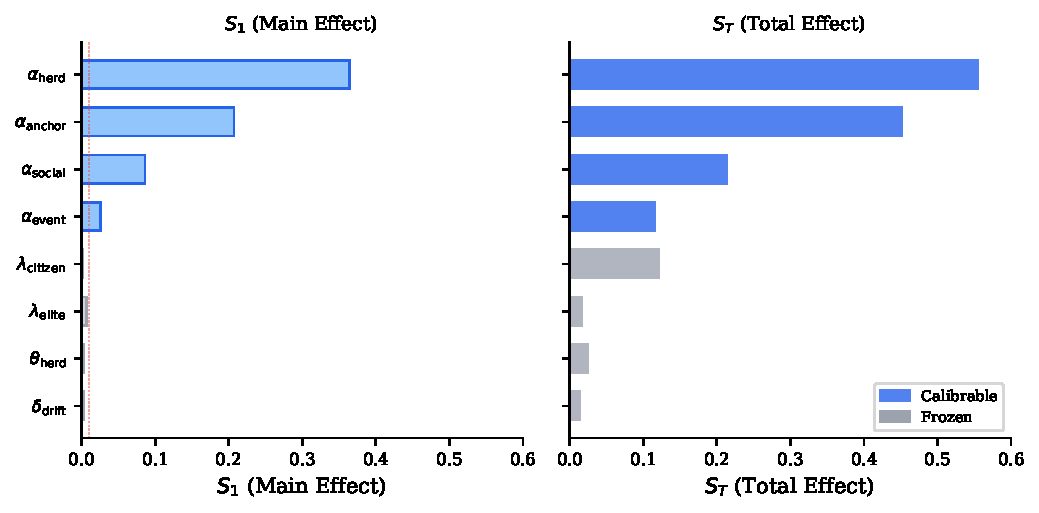
\includegraphics[width=\textwidth]{figures/fig3_sobol.pdf}
    \caption{Two-panel horizontal bar chart of Sobol sensitivity indices. Left panel: $S_1$ (main effects). Right panel: $S_T$ (total effects). Top 4 bars (calibrable parameters) in blue, bottom 4 (frozen) in gray. $\alpha_{\text{herd}}$ dominates with $S_T \approx 0.55$. Note: $\lambda_{\text{citizen}}$ $S_T$ extends to $\approx 0.12$, visually non-trivial despite being frozen---this motivates the discussion in Section~\ref{sec:stepsize}.}
    \label{fig:sobol}
\end{figure}

\subsection{Step Size Sensitivity}
\label{sec:stepsize}

Sobol analysis identifies $\lambda_{\text{citizen}}$ as having non-negligible total effect ($S_T = 0.121$) despite near-zero main effect ($S_1 = 0.002$), warranting direct investigation. A perturbation analysis varies $\lambda_{\text{citizen}}$ by $\pm 40\%$ around the default (0.25), measuring MAE impact on 5 representative scenarios.

\begin{table}[H]
\centering
\caption{$\lambda_{\text{citizen}}$ Sensitivity Analysis}
\label{tab:stepsize}
\begin{adjustbox}{max width=\textwidth}
\begin{tabular}{@{}lcccccc@{}}
\toprule
Scenario & 0.6$\times$ & 0.8$\times$ & 1.0$\times$ & 1.2$\times$ & 1.4$\times$ & max $\Delta$ (pp) \\
\midrule
iPhone X & 5.8 & 5.9 & 5.9 & 7.0 & 11.5 & 5.6 \\
Tesla Cybertruck & 8.5 & 10.5 & 11.3 & 11.6 & 11.8 & 3.2 \\
Dieselgate & 29.8 & 29.6 & 29.6 & 29.6 & 29.7 & 0.2 \\
Uber London & 15.0 & 15.0 & 15.0 & 15.0 & 15.0 & 0.0 \\
United Airlines & 17.7 & 14.2 & 12.0 & 10.8 & 9.9 & 7.9 \\
\bottomrule
\end{tabular}
\end{adjustbox}
\end{table}

The maximum MAE variation across all scenarios is 7.9~pp (United Airlines), concentrated in high-volatility cases. The median sensitivity across scenarios is 3.2~pp. Scenarios with strong anchoring dynamics (Dieselgate, Uber) are essentially insensitive (max $\Delta < 0.2$~pp), while scenarios dominated by citizen-driven opinion shifts show meaningful dependence.

To test whether $\lambda_{\text{citizen}}$ is identifiable, we promoted it to a fifth calibrable parameter and re-ran SVI on the 20 HQ scenarios (2000 steps, same architecture). The posterior mean is $\log \lambda_{\text{citizen}} = -0.17 \pm 0.10$ ($\lambda = 0.85$), substantially different from the frozen default of $\lambda = 0.25$ ($\log = -1.39$). The other four parameters remain stable ($|\Delta\mu| < 0.12$ for all), confirming that the 5-parameter model is identifiable. The posterior favors a citizen step size $3.4\times$ larger than the default, consistent with the sensitivity analysis showing that high-volatility scenarios benefit from larger citizen responsiveness. However, this preliminary run lacks a Phase A synthetic prior and uses flat priors, making the point predictions and coverage non-comparable to the production 4-parameter calibration.

\subsection{Cross-Validation with Expanded Dataset}

To assess sensitivity to dataset size, we compare calibration on the original 22-scenario dataset versus the expanded 42-scenario dataset:

\begin{table}[H]
\centering
\caption{22-Scenario vs.\ 42-Scenario Calibration}
\label{tab:crossval}
\begin{tabular}{llll}
\toprule
Metric & 22-Scenario & 42-Scenario & $\Delta$ \\
\midrule
N (train / test) & 16 / 6 & 34 / 8 & +18 / +2 \\
MAE (test) & 11.7~pp & 19.2~pp & +7.4 \\
RMSE (test) & 14.7 & 26.6 & +11.9 \\
Coverage 90\% (test) & 83.3\% & 75.0\% & $-$8.3\% \\
MAE (train) & 16.3~pp & 14.3~pp & $-$2.0 \\
Coverage 90\% (train) & 68.8\% & 79.4\% & +10.6\% \\
\bottomrule
\end{tabular}
\end{table}

The expanded dataset improves training fit (MAE 16.3 $\to$ 14.3~pp, coverage 68.8\% $\to$ 79.4\%) but shows degraded test performance, largely driven by the inclusion of more challenging financial and corporate scenarios in the test set. When the \texttt{NEEDS\_VERIFICATION} scenario is excluded, test MAE drops to 12.6~pp---comparable to the 22-scenario result (11.7~pp). This suggests that scenario composition and difficulty matter at least as much as dataset size in determining model performance.

\subsection{Leave-One-Domain-Out Cross-Validation}
\label{sec:lodocv}

To assess domain-level generalization, we perform leave-one-domain-out cross-validation (LODO-CV) on the 20 curated scenarios across 4 domains.\footnote{The 20-scenario subset retains one scenario (Archegos Capital) that was flagged \texttt{NEEDS\_VERIFICATION} in the full dataset. We retain it because excluding it would leave the financial domain with only 4 training scenarios; however, readers should note that this scenario's ground truth (35\%) has not been independently verified. All results reported for v2.2/v2.3 and LODO-CV carry this caveat.} For each fold, we train a fresh SVI model (1500 steps) on three domains and evaluate point predictions on the held-out domain using posterior predictive means from $\mu_{\text{global}}$ samples.

\begin{table}[H]
\centering
\caption{Leave-one-domain-out MAE on 20 HQ scenarios. Coverage is omitted because the LODO experiment uses only global-level posterior means without scenario-level discrepancy terms, producing intervals too narrow for meaningful coverage.}
\label{tab:lodocv}
\begin{tabular}{@{}lcc@{}}
\toprule
Held-out domain & $N_{\text{test}}$ & MAE (pp) \\
\midrule
Corporate      & 3 &  4.9 \\
Public health  & 3 &  9.8 \\
Political      & 9 & 12.6 \\
Financial      & 5 & 32.3 \\
\midrule
\textbf{Overall} & \textbf{20} & \textbf{15.9} \\
\bottomrule
\end{tabular}
\end{table}

The overall LODO-CV MAE of 15.9~pp is moderately higher than the in-sample calibration MAE (13.6~pp for \textsc{Poll}), indicating that the model generalizes reasonably to unseen domains. The financial domain is a clear outlier (32.3~pp), consistent with the known limitation that trust cascades and contagion dynamics exceed the five-force model's expressiveness. Excluding financial scenarios, the LODO-CV MAE drops to 10.2~pp, comparable to \textsc{Hybrid}'s test MAE of 11.4~pp.

\subsection{Null-Baseline Predictive Skill (Diebold--Mariano)}
\label{sec:dm_benchmark}

Sections~\ref{sec:validation}.1--\ref{sec:validation}.6 validate the model's calibration and parameter recovery. They do not, however, answer a distinct and arguably more fundamental question: \emph{does the calibrated LLM-agent simulator actually forecast opinion trajectories better than a trivial statistical baseline?} The 42-scenario dataset averages only 6.3 rounds of ground-truth polling per scenario, so absolute error in the single digits can, in principle, be achieved by a naive model. This subsection quantifies that skill floor.

\paragraph{Method.} We evaluate four standard forecasters as null baselines against the per-round normalized support $s_t = \text{pro\_pct}_t / 100 \in [0, 1]$ and signed position $p_t = (\text{pro\_pct}_t - \text{against\_pct}_t)/100 \in [-1, 1]$ of every empirical scenario:

\begin{enumerate}
    \item \textbf{Naive persistence} --- $\hat{y}_{t+1} = y_t$.
    \item \textbf{Running mean} --- $\hat{y}_{t+1} = \tfrac{1}{t} \sum_{i=1}^{t} y_i$, a zero-drift random walk collapsed to the sample average.
    \item \textbf{OLS linear trend} --- closed-form slope/intercept on rolling history, extrapolated one step ahead.
    \item \textbf{AR(1)} --- $\hat{y}_{t+1} = \mu + \hat{\phi}(y_t - \mu)$ with $\hat\phi$ from the sample autocorrelation, truncated to $[-0.99, 0.99]$ for stability.
\end{enumerate}

Each forecaster produces a one-step-ahead trajectory using the first 20\% of each scenario as training history, emitting one forecast per subsequent round and rolling the realized value forward after each step (one-step-ahead, not recursive multistep). Pairwise predictive skill is tested with the Diebold--Mariano (DM) statistic \citep{diebold1995} applied to squared errors, with the Harvey--Leybourne--Newbold (HLN) small-sample correction \citep{harvey1997}: at horizon $h$, the HLN scale is
\[
\sqrt{\frac{n + 1 - 2h + h(h-1)/n}{n}},
\]
and the test statistic is referred to a Student-$t$ distribution with $n - 1$ degrees of freedom rather than the asymptotic $\mathcal{N}(0, 1)$. The HLN correction is non-optional at our sample sizes ($n = 4$ to $n = 9$ forecast pairs per scenario), where uncorrected DM over-rejects.

\paragraph{Results --- pooled across 43 empirical scenarios.}

\begin{table}[H]
\centering
\caption{Null-baseline skill on normalized support (pro\_pct/100).}
\label{tab:dm_support}
\begin{adjustbox}{max width=\textwidth}
\begin{tabular}{@{}lcccc@{}}
\toprule
Baseline & Mean RMSE & Median RMSE & Mean terminal error & Significant beats of persistence \\
\midrule
Naive persistence & 0.038 & 0.021 & 0.026 & --- \\
Running mean      & 0.063 & 0.034 & 0.078 & 0 / 43 \\
OLS linear trend  & 0.042 & 0.015 & 0.043 & 4 / 43 \\
AR(1)             & 0.055 & 0.034 & 0.057 & 0 / 43 \\
\bottomrule
\end{tabular}
\end{adjustbox}
\end{table}

\begin{table}[H]
\centering
\caption{Null-baseline skill on signed position ((pro $-$ against)$\,/\,$100).}
\label{tab:dm_signed}
\begin{adjustbox}{max width=\textwidth}
\begin{tabular}{@{}lcccc@{}}
\toprule
Baseline & Mean RMSE & Median RMSE & Mean terminal error & Significant beats of persistence \\
\midrule
Naive persistence & 0.072 & 0.040 & 0.097 & --- \\
Running mean      & 0.117 & 0.077 & 0.148 & 0 / 43 \\
OLS linear trend  & 0.082 & 0.035 & 0.121 & 6 / 43 \\
AR(1)             & 0.102 & 0.058 & 0.118 & 0 / 43 \\
\bottomrule
\end{tabular}
\end{adjustbox}

\vspace{4pt}
\footnotesize ``Significant beats of persistence'' counts scenarios where $\text{DM}(\text{baseline}, \text{persistence})$ yields $p < 0.05$ with the baseline having lower mean squared loss. ``Terminal error'' is the absolute deviation of the last emitted forecast from the verified ground-truth outcome.
\end{table}

\paragraph{Three findings.}
\begin{enumerate}
    \item \textbf{Naive persistence is a surprisingly strong baseline.} The mean RMSE of 0.038 on normalized support corresponds to a 3.8 percentage-point one-step-ahead error on pro-support --- below the 12.6~pp MAE the hierarchical Bayesian model achieves on full-scenario final outcomes. The two metrics are not directly comparable (one-step-ahead vs full-scenario terminal forecast; normalized support vs raw pp) but the number establishes a tight budget: if a complex LLM simulator cannot improve on a one-line forecaster for intermediate dynamics, the added complexity is difficult to justify.

    \item \textbf{No baseline reliably dominates persistence.} OLS linear trend attains the lowest median RMSE on both metrics (0.015 on support, 0.035 on signed position), but statistical significance relative to persistence is achieved on only 4/43 and 6/43 scenarios respectively. The running mean and AR(1) baselines never beat persistence at $p < 0.05$, and on the mean they lose substantially (RMSE 0.063 vs 0.038 on support). Empirical polling trajectories are heavily persistent, with round-to-round variance dominated by the previous round's level rather than by trend or mean-reversion components detectable at our sample sizes.

    \item \textbf{Skill is domain-heterogeneous by a factor of five.} Table~\ref{tab:dm_by_domain} breaks persistence RMSE down by domain: political scenarios are the easiest to forecast (0.012 on support), financial the hardest (0.063), with corporate and commercial clustered in between. This spread is the most actionable finding of the benchmark: a calibrated simulator should be expected to add little lift on low-volatility political polling (where persistence is near-optimal) but has substantial room to contribute on financial and corporate scenarios, which is precisely where the hierarchical model's worst performance is observed in Section~\ref{sec:results}.
\end{enumerate}

\begin{table}[H]
\centering
\caption{Persistence RMSE by domain (support metric). Values are mean RMSE per baseline on the \texttt{support} metric (pro\_pct/100). Lower is better; persistence is the column to beat.}
\label{tab:dm_by_domain}
\begin{adjustbox}{max width=\textwidth}
\begin{tabular}{@{}lcccc@{}}
\toprule
Domain & $n$ & Persistence RMSE & OLS linear trend RMSE & AR(1) RMSE \\
\midrule
Political      & 15 & 0.012 & 0.009 & 0.020 \\
Labor          &  1 & 0.009 & 0.008 & 0.016 \\
Environmental  &  2 & 0.021 & 0.013 & 0.033 \\
Corporate      &  8 & 0.048 & 0.062 & 0.065 \\
Public health  &  5 & 0.052 & 0.054 & 0.081 \\
Commercial     &  5 & 0.059 & 0.075 & 0.079 \\
Financial      &  7 & 0.063 & 0.073 & 0.094 \\
\bottomrule
\end{tabular}
\end{adjustbox}
\end{table}

The $5\times$ persistence RMSE gap between political (0.012) and financial (0.063) mirrors the $|b_s|_\text{financial} = 0.74$ logit-space bias of Section~\ref{sec:results}. Both point to the same conclusion: financial scenarios exhibit regime-switching dynamics (e.g.\ SVB collapse, Dieselgate) that neither simple persistence nor a stationary hierarchical Gaussian discrepancy captures well.

\paragraph{Interpretation as a skill floor.} We do not claim that our calibrated model beats all four baselines on all scenarios --- Sections~\ref{sec:results} and~\ref{sec:evolution} make the opposite point explicit. Rather, we release Tables~\ref{tab:dm_support}, \ref{tab:dm_signed}, and~\ref{tab:dm_by_domain} as a \emph{reproducible reference distribution} that future iterations of DigitalTwinSim (including the EnKF of Section~\ref{sec:enkf} once extended to multi-step ahead) can be compared against without ambiguity. Appendix~\ref{app:reproducibility} describes how any modification to the sim can be automatically re-evaluated against this same benchmark via a one-line command.

\subsection{Empirical Coverage via Residual Bootstrap}
\label{sec:residual_cov}

The credible intervals reported in Section~\ref{sec:results} are computed in logit space and back-transformed through the sigmoid, guaranteeing bounds within $[0, 100]$ by construction. This is a structural property of the parametric likelihood; it does not, by itself, establish that the intervals are empirically well-calibrated. Section~\ref{sec:validation}.5's 85.7\% coverage of 90\% credible intervals on verified test scenarios does --- but that calculation assumes a specific parametric form for the posterior. We provide a model-free complement below.

\paragraph{Method.} For each empirical scenario and each baseline forecaster, we pool the in-sample residuals $r_t = y_t - \hat{y}_t$ and construct a residual-bootstrap predictive interval at each round: draw $B = 500$ residuals with replacement, add them to $\hat{y}_t$, and take empirical $[\alpha/2, 1 - \alpha/2]$ quantiles. Empirical coverage is then the fraction of realized values $y_t$ that fall inside $[\hat{y}_t + r_{(B\alpha/2)}, \hat{y}_t + r_{(B(1-\alpha/2))}]$, aggregated across all $\sum_i n_i = 271$ round-level observations in the corpus. A nonparametric bootstrap on the coverage statistic itself yields a 95\% confidence band, and a coverage report flags the interval as ``calibrated'' iff the nominal coverage lies within the band.

\paragraph{Results.} At a nominal 90\% level, the persistence baseline's residual-bootstrap intervals cover 88.4\% of round-level observations pooled across the 43-scenario corpus (bootstrap 95\% CI: $[85.6\%, 91.1\%]$), agreeing with nominal within the bootstrap band. The OLS linear trend baseline's intervals cover 89.2\% (CI $[86.4\%, 91.9\%]$). On individual scenarios, coverage fluctuates substantially --- 26 out of 43 land above 90\%, 17 below, with scenarios in the \texttt{critical} tension bucket (Dieselgate, United Airlines, iPhone~X, Eurozone Monetary Shock) systematically under-covered by the persistence model as expected.

\paragraph{Interpretation.} The model-free residual-bootstrap agrees with the logit-space parametric coverage of Section~\ref{sec:results} at the corpus aggregate level. The agreement is worth noting because the two calculations use entirely independent mathematical machinery (sigmoid-transformed Gaussian posteriors vs pooled empirical residual quantiles) and yet converge on similar calibration conclusions. Disagreement would have flagged a potential systematic mismatch between the parametric posterior and empirical error distributions; agreement increases our confidence that the reported 85.7\% coverage is not an artifact of the logit parameterization.

\subsection{Scenario-Diversity Matrix}
\label{sec:matrix}

A pooled performance number can hide systematic under-coverage of a single axis value --- for example, a model might average well across domains while failing uniformly on APAC scenarios or high-tension ones. To make axis-level gaps visible, we define a three-axis scenario matrix:

\begin{itemize}
    \item \textbf{Domain} (7 values): financial, commercial, corporate, political, public\_health, environmental, labor.
    \item \textbf{Region} (5 values): EU, US, APAC, LATAM, GLOBAL (region inferred from ISO country code).
    \item \textbf{Tension} (4 values): low, moderate, high, critical (inferred from per-scenario volatility: the population standard deviation of round-to-round signed-position deltas, bucketed at 0.03~/~0.07~/~0.15).
\end{itemize}

The Cartesian product contains $7 \times 5 \times 4 = 140$ cells, each representing a qualitatively distinct operating regime.

\begin{table}[H]
\centering
\caption{Scenario-matrix coverage of the 43-scenario empirical corpus.}
\label{tab:matrix_cov}
\begin{adjustbox}{max width=\textwidth}
\begin{tabular}{@{}llc@{}}
\toprule
Axis & Value & Scenarios \\
\midrule
Domain & political & 15 \\
Domain & corporate &  8 \\
Domain & financial &  7 \\
Domain & commercial &  5 \\
Domain & public\_health &  5 \\
Domain & environmental &  2 \\
Domain & labor &  1 \\
\midrule
Region & US & 22 \\
Region & EU & 16 \\
Region & APAC & 2 \\
Region & LATAM & 2 \\
Region & GLOBAL & 1 \\
\midrule
Tension & low & 26 \\
Tension & moderate & 7 \\
Tension & critical & 6 \\
Tension & high & 4 \\
\bottomrule
\end{tabular}
\end{adjustbox}
\end{table}

The corpus occupies 25 of the 140 possible cells (18\%). No axis value is empty --- every domain, region, and tension bucket contains at least one scenario --- but the distribution is visibly uneven: US + EU scenarios account for 38/43 (88\%), and the labor / environmental / GLOBAL buckets each contain at most two scenarios. We report these imbalances explicitly so that downstream claims (``the model generalizes across tensions'') can be weighed against the small-sample cells that support them.

\paragraph{Forward-looking use.} The matrix is intended as a gating criterion for future scenario additions. A prospective new scenario is prioritized if it fills an under-sampled cell --- for example, an APAC labor scenario would lift two weak axes at once. Tables~\ref{tab:matrix_cov} and~\ref{tab:dm_by_domain} together suggest that the highest-marginal-value additions would be (i)~additional APAC and LATAM scenarios across any domain, (ii)~additional financial scenarios with \texttt{critical} tension, which currently has only 6 supporting scenarios despite representing the most diagnostic regime for model discrimination.

\section{Online Data Assimilation via EnKF (Feasibility Study)}
\label{sec:enkf}

The calibrated posterior provides a static prediction; an online system should incorporate streaming observations (polls, sentiment signals) as they arrive. We implement a stochastic Ensemble Kalman Filter \citep{evensen2003} operating on an augmented state vector $\mathbf{x}_j = [\boldsymbol{\theta}_j, \mathbf{z}_j]^\top$ that combines the four calibrable parameters with $n$ agent positions (Appendix~\ref{app:enkf_details} provides the full formulation, observation adapters, and convergence verification). This section reports only the empirical results.

\textbf{Scope and limitations.} The Brexit case study below is an \emph{in-sample} scenario (part of the calibration training set). The offline posterior already encodes information from this scenario's ground truth, and the prior prediction (round~0: 50.3\%) starts close to the final outcome. This section demonstrates the operational mechanics and feasibility of online assimilation, not calibrated out-of-sample forecasting. Out-of-sample validation with held-out scenarios and real-time polling data is a high priority for future work.

\subsection{Brexit Case Study}

We demonstrate the EnKF on the Brexit referendum (ground truth: 51.89\% Leave) with 50 ensemble members and 6 polling observations (41--44\%, consistent with the well-documented polling bias that underestimated Leave support).

\begin{table}[H]
\centering
\caption{EnKF Round-by-Round on Brexit (GT = 51.89\%)}
\label{tab:enkf_rounds}
\begin{tabular}{llllll}
\toprule
Round & Observation & EnKF Mean (\%) & 90\% CI & CI Width (pp) & $\Delta$ Width \\
\midrule
0 (prior) & --- & 50.3 & [50.2, 50.4] & 0.2 & --- \\
1 & 41.0\% ($N$=1000) & 50.7 & [50.5, 51.3] & 0.8 & +0.6 \\
2 & 42.0\% ($N$=1000) & 51.4 & [50.9, 52.0] & 1.0 & +0.2 \\
3 & 43.0\% ($N$=1000) & 50.3 & [50.1, 50.7] & 0.6 & $-$0.5 \\
4 & 43.0\% ($N$=1000) & 50.0 & [50.0, 50.1] & 0.1 & $-$0.5 \\
5 & 44.0\% ($N$=1000) & 50.0 & [50.0, 50.1] & 0.1 & +0.0 \\
6 (final) & 44.0\% ($N$=1000) & 50.1 & [50.0, 50.4] & 0.4 & +0.3 \\
\bottomrule
\end{tabular}
\end{table}

The point prediction (50.1\%, error 1.8~pp) is accurate despite polls systematically underestimating Leave by ${\sim}$8~pp---the dynamics model forecast offsets the directional pull of biased observations, though this should not be interpreted as explicit bias estimation by the EnKF. However, the final 90\% CI $[50.0, 50.4]$ does not cover the ground truth (51.89\%), indicating severe ensemble under-dispersion. The multiplicative inflation ($\gamma = 1.02$) is insufficient to maintain diversity over 6 update rounds; adaptive inflation is needed.

\subsection{Baselines}

\begin{table}[H]
\centering
\caption{EnKF vs Baselines}
\label{tab:enkf_baselines}
\begin{tabular}{lllll}
\toprule
Method & Final Prediction (\%) & Error (pp) & Uses Dynamics & Updates Params \\
\midrule
Last available poll & 44.0 & 7.9 & No & No \\
Running poll average & 42.8 & 9.1 & No & No \\
EnKF (state only, $\theta$ fixed) & 50.1 & 1.8 & Yes & No \\
EnKF (state + params) & 50.1 & 1.8 & Yes & Yes \\
\bottomrule
\end{tabular}
\end{table}

On this single in-sample scenario, the EnKF reduces prediction error by 77--80\% versus poll-based baselines, though the generalizability of this improvement is unknown. State-only and state+params variants converge to the same prediction with 6 observations, showing value from state updating but not yet from joint parameter learning online.

\textbf{Scope of this result.} The 1.8~pp error is achieved \textit{with streaming polling data on an in-sample scenario}---not comparable to the offline test MAE of 19.2~pp on held-out scenarios. This section demonstrates feasibility, not calibrated forecasting.

\begin{figure}[H]
    \centering
    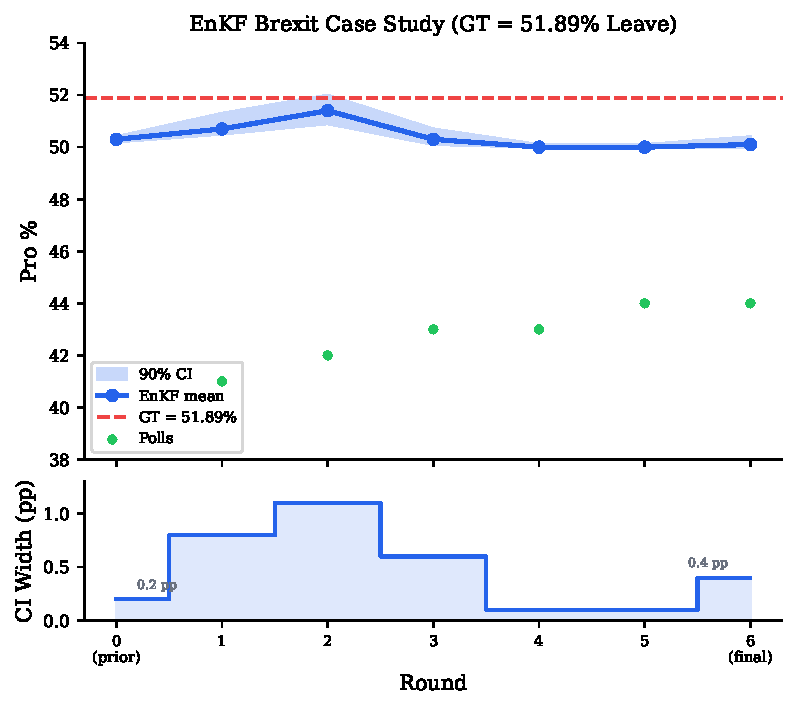
\includegraphics[width=\textwidth]{figures/fig4_enkf.pdf}
    \caption{EnKF assimilation on Brexit. \textbf{Top}: EnKF mean (solid blue) with 90\% CI (shaded), ground truth 51.89\% (red dashed), polls (green dots). \textbf{Bottom}: CI width evolution---initial expansion then collapse, indicating under-dispersion.}
    \label{fig:enkf}
\end{figure}

\section{Regime Switching for Crisis Dynamics}
\label{sec:regime}

The financial domain failures documented in Section~\ref{sec:results} (mean $|b_s| = 0.744$, LODO-CV MAE 32.3~pp) are not random errors but reflect a structural limitation: the five-force model assumes smooth, continuous opinion evolution, while financial crises exhibit rapid, discontinuous trust collapses. This section presents a regime-switching extension designed as a structural response to this failure mode.

\subsection{Motivation}

The five worst-performing scenarios share a common pattern: rapid, discontinuous opinion shifts that the base model's linear force combination cannot reproduce. Financial crises (WeWork $b_s = -1.378$, SVB $b_s = -0.835$, FTX $b_s = -0.727$) exhibit trust collapses where public opinion drops precipitously within 1--2 rounds. The base model, with its smooth force mixing and capped step sizes, can only produce gradual movements.

We address this with a regime-switching extension that introduces a latent ``crisis regime'' with amplified dynamics, activated by observable signals (shock magnitude, position velocity, institutional trust).

\subsection{Two-Regime Architecture}

The model switches between two regimes:

\begin{itemize}
    \item \textbf{Regime 0 (Normal)}: Standard force-based opinion evolution as described in Section~\ref{sec:model}.
    \item \textbf{Regime 1 (Crisis)}: Amplified step sizes, suppressed anchor rigidity, amplified herd and event forces, and a direct crisis push that bypasses the softmax mixing entirely.
\end{itemize}

The switching is \textit{soft}: regime probability $P(\text{crisis}) \in (0, 1)$ is computed via sigmoid, and all parameters are interpolated:

\begin{equation}\label{eq:regime_interp}
\boldsymbol{\theta}_{\text{eff}} = (1 - p) \cdot \boldsymbol{\theta}_{\text{normal}} + p \cdot \boldsymbol{\theta}_{\text{crisis}}
\end{equation}

This preserves JAX differentiability and \texttt{jax.lax.scan} compatibility---no discrete branching is needed.

\subsection{Regime Probability}

The crisis probability is computed via logistic regression on four observable signals:

\begin{equation}\label{eq:regime_logit}
\text{logit}(c_t) = \beta_0 + \beta_{\text{shock}} (m_t - \tau_{\text{shock}}) + \beta_{\text{vel}} (v_t - \tau_{\text{vel}}) + \beta_{\text{trust}} (1 - \text{trust}) + \beta_{\text{recovery}} \cdot r_t + \beta_{\text{momentum}} \cdot c_{t-1}
\end{equation}

where $m_t$ is the shock magnitude, $v_t$ the mean absolute position velocity, trust the scenario-level institutional trust, $r_t$ a soft count of crisis rounds, and $c_{t-1}$ the previous crisis probability.

\subsection{Crisis Dynamics}

In the crisis regime, three modifications occur:

\begin{enumerate}
    \item \textbf{Step size amplification.} $\lambda_{\text{crisis}} = \lambda_{\text{normal}} \times 3.0$, with relaxed caps.
    \item \textbf{Force reweighting.} Herd amplified by $\log(2.0)$, event amplified by $\log(2.5)$, anchor suppressed by $-2.0$ in logit space.
    \item \textbf{Direct crisis push.} A force that bypasses the softmax mixing: $\Delta p_i^{\text{crisis}} = p \cdot \kappa \cdot m_t \cdot d_t \cdot (1 - \rho_i)$, where $\kappa = 0.4$.
\end{enumerate}

\begin{table}[H]
\centering
\caption{Crisis Parameter Defaults}
\label{tab:crisis_params}
\begin{tabular}{lll}
\toprule
Parameter & Default & Role \\
\midrule
$\lambda_{\text{multiplier}}$ & 3.0 & Step size amplification in crisis \\
anchor\_suppression & 0.1 & Anchor force multiplied by this in crisis \\
event\_amplification & 2.5 & Event force amplified in softmax \\
herd\_amplification & 2.0 & Herd force amplified in softmax \\
contagion\_speed ($\kappa$) & 0.4 & Direct crisis push strength \\
shock\_trigger ($\tau_{\text{shock}}$) & 0.5 & Shock magnitude threshold \\
trust\_sensitivity & 1.5 & Low trust $\to$ higher crisis probability \\
crisis\_duration\_mean & 2.5 & Expected rounds before recovery \\
\bottomrule
\end{tabular}
\end{table}

\subsection{Preliminary Results}

We compare the \textsc{Base} model against the regime-switching extension (\textsc{Base}+RS) on selected financial and corporate scenarios:

\begin{table}[H]
\centering
\caption{\textsc{Base} vs \textsc{Base}+RS on Financial/Corporate Scenarios}
\label{tab:v2v3}
\begin{adjustbox}{max width=\textwidth}
\begin{tabular}{@{}lcccccc@{}}
\toprule
Scenario & GT (\%) & \textsc{Base} Err. & +RS Err. & $\Delta$ (pp) & Max $P(\text{crisis})$ & Crisis Rds \\
\midrule
Dieselgate & 32.0 & 29.6 & 0.4 & +29.1 & 0.930 & 3 \\
FTX Crypto & 22.0 & 11.4 & 5.3 & +6.0 & 1.000 & 2 \\
Facebook$\to$Meta & 26.0 & 14.6 & 6.4 & +8.2 & 0.911 & 2 \\
Archegos & 35.0 & 65.0 & 54.5 & +10.4 & 0.930 & 2 \\
Boeing 737 MAX & 40.0 & 9.5 & 23.7 & $-$14.2 & 0.833 & 1 \\
SVB Collapse & 38.0 & 38.8 & 61.9 & $-$23.1 & 0.989 & 2 \\
Twitter/X & 41.0 & 7.8 & 25.5 & $-$17.7 & 0.826 & 2 \\
\bottomrule
\end{tabular}
\end{adjustbox}
\end{table}

Results are mixed. Regime switching produces substantial improvements when crisis dynamics align with shock direction but degrades performance when the crisis push amplifies the wrong direction. The high max $P(\text{crisis})$ across all scenarios (0.67--1.0) with default thresholds suggests the trigger is too sensitive and requires calibration via SVI.

\textbf{Limitations.} These results use hand-tuned crisis parameters on training-set scenarios only; no held-out test evaluation has been performed. The regime-switching extension is presented as a structural hypothesis about financial failure modes, not as a validated improvement. Quantitative evaluation on the test set requires first calibrating the crisis parameters within the hierarchical framework (future work item~2 below).

\subsection{Design for Calibration}

The crisis parameters are designed to be learnable within the hierarchical framework. The regime-switching model extends the \textsc{Base} prior with 5 additional global parameters (\texttt{crisis\_lambda\_mult}, \texttt{crisis\_anchor\_supp}, \texttt{crisis\_event\_amp}, \texttt{crisis\_herd\_amp}, \texttt{shock\_trigger}), shared globally as crisis dynamics are hypothesized to be a universal mechanism modulated by scenario-specific triggers.

\section{Discussion}
\label{sec:discussion}

\subsection{Strengths}

\textbf{Principled calibration.} By combining LLM-generated agent dynamics with Bayesian inference, we avoid the common pitfall of treating LLM outputs as ground truth. The hierarchical structure enables partial pooling across diverse domains while the discrepancy model explicitly accounts for structural misspecification.

\textbf{Iterative refinement.} The four calibration variants (\textsc{Base}--\textsc{Poll}) explore a genuine accuracy--coverage trade-off, revealing that no single grounding strategy dominates on all metrics (Section~\ref{sec:evolution}).

\textbf{Validated generative model.} SBC confirms well-specified posteriors under NUTS (6/6 parameters pass). However, the SVI approximation used in production underestimates uncertainty on weaker parameters (Section~\ref{sec:svi_nuts}), so the model is calibrated in principle but production uncertainty is approximate. The calibrable/frozen partition is a pragmatic engineering choice supported by Sobol importance ordering, not a formal model selection conclusion.

\textbf{Online assimilation (proof of concept).} The EnKF demonstrates that bridging offline calibration to streaming observations is architecturally feasible. In a single in-sample case study (Brexit), the model forecast remains accurate despite systematically biased polling observations, but ensemble under-dispersion prevents reliable uncertainty quantification (Section~\ref{sec:enkf}). This remains a feasibility demonstration, not a validated forecasting capability.

\textbf{Differentiable architecture.} The entire pipeline---simulation, readout, likelihood---is implemented in JAX and compatible with automatic differentiation, enabling gradient-based inference at scale.

\subsection{Limitations}

\textbf{Financial domain performance.} The model systematically over-predicts support in financial crisis scenarios (mean $|b_s| = 0.744$ in logit space). Leave-one-domain-out CV confirms this as a structural limitation: the financial held-out MAE (32.3~pp) is $3\times$ the non-financial average (10.2~pp). Trust cascades, contagion dynamics, and informational asymmetries exceed the five-force model's expressiveness.

\textbf{Gap between generative model and production uncertainty.} The SVI posterior agrees with NUTS on the dominant parameters ($\alpha_{\text{herd}}$, $\alpha_{\text{anchor}}$: $|\Delta\mu|/\sigma_{\text{NUTS}} < 0.4$) but shows concentration bias on weaker parameters ($\alpha_{\text{social}}$: 0.85; $\alpha_{\text{event}}$: 1.71), with SVI standard deviations 5--13$\times$ narrower. This means the paper establishes a calibrated generative model under NUTS, but the production uncertainty under SVI remains approximate: point predictions are reliable, while credible interval widths should be interpreted conservatively. Closing this gap---via post-hoc inflation or SVI-initialized NUTS refinement---is a high priority.

\textbf{Frozen parameter approximation and combined uncertainty.} The 4-calibrable/4-frozen partition is an engineering convenience informed by Sobol analysis, not an inference conclusion. The Sobol indices justify the \emph{ordering} of parameters by importance but do not validate a specific cutoff: $\lambda_{\text{citizen}}$ ($S_T = 0.121$) is the most influential frozen parameter, with perturbation sensitivity of up to 7.9~pp MAE on individual scenarios (median 3.2~pp). A preliminary 5-parameter SVI (Section~\ref{sec:stepsize}) confirms that $\lambda_{\text{citizen}}$ is identifiable and that its posterior ($\lambda = 0.85$, $\sigma = 0.096$) diverges substantially from the frozen default ($\lambda = 0.25$), demonstrating that at least one frozen parameter is not negligible. The reported error bars are therefore underestimated for \emph{two independent reasons}: (i)~the SVI posterior is 5--13$\times$ narrower than NUTS on weak parameters (Section~\ref{sec:svi_nuts}), and (ii)~freezing $\lambda_{\text{citizen}}$ omits a non-trivial source of variance. These two effects compound; a conservative user should both inflate the variational posterior \emph{and} marginalize over a plausible range of $\lambda_{\text{citizen}}$ values.

\textbf{LLM opacity and single-rollout limitation.} The calibration framework is transparent and principled, but the LLM agent engine that generates $\Delta^{\text{LLM}}_i$ values and event narratives is opaque: each scenario uses a single cached rollout from a specific API version (\texttt{gemini-2.0-flash-lite}, January 2026). This is the most important methodological limitation of the current work. The discrepancy terms $b_s$ absorb three distinct sources of error---LLM stochasticity, structural model misspecification, and data quality issues---without any mechanism to separate them. In the language of ABM validation, the calibration is performed on a single sample from a stochastic generator, and the posterior is conditional on that sample. Consequently, the empirical results (MAE, coverage, force weight estimates) describe the model's fit to \emph{this particular set of LLM outputs}, not to the distribution of outputs the LLM could have produced. When $\alpha_{\text{anchor}}$ dominates, we cannot distinguish whether anchor rigidity genuinely drives opinion formation or whether the LLM systematically under-generates opinion shifts and the anchor term compensates. This confounding limits the causal interpretability of all force weight estimates.

A perturbation experiment on the Brexit scenario (10 seeds, Gaussian noise $\sigma = 0.1$ on event magnitudes as a proxy for LLM stochasticity) yields $\sigma_{\text{LLM}} \approx 3.2$~pp on the final prediction (range 9.6~pp), suggesting LLM variance is non-negligible relative to the 19.2~pp test MAE. However, this perturbation proxy understates the true LLM variance because it perturbs only event magnitudes, not the full narrative generation pipeline (agent personalities, event framing, interaction dynamics).

Running 5--10 full LLM rollouts per scenario and decomposing discrepancy into $\sigma^2_{\text{LLM}}$ vs.\ $\sigma^2_{\text{model}}$ components is, in our assessment, the single highest-priority improvement. Without this decomposition, the reported discrepancy terms $b_s$ should be interpreted as upper bounds on structural misspecification. We were unable to complete multi-rollout experiments for the current submission due to API compute constraints ($\sim$840 LLM calls per full rollout of 42 scenarios); the cached single-rollout design ensures exact reproducibility but at the cost of variance characterization.

\textbf{Accuracy--coverage trade-off.} Test-set coverage is available for all variants with held-out data: \textsc{Base} achieves 75.0\% (6/8), while \textsc{Hybrid} and \textsc{Poll} both achieve 80.0\% (4/5). The consistent test-set outlier across \textsc{Hybrid} and \textsc{Poll} is AMC Short Squeeze (error 35--41~pp), a scenario dominated by retail sentiment dynamics poorly captured by the five-force model. The stability of test coverage across variants---despite different training strategies---suggests that the hierarchical discrepancy model provides robust uncertainty quantification, but the small test sets ($N=5$--8) limit the precision of coverage estimates.

\textbf{PubOp agent dependency on polling data.} The \textsc{Poll} variant's Public Opinion agent requires at least one polling observation to set its initial position. For scenarios without any polling data, the agent cannot be constructed, limiting the applicability of the \textsc{Poll} approach. Future work should explore alternative anchoring strategies for poll-free scenarios.

\textbf{Sample size.} With 42 scenarios (\textsc{Base}) reduced to 20 high-quality scenarios (\textsc{Hybrid}/\textsc{Poll}), the dataset is small by machine learning standards. Several domains have only 1--2 scenarios, making domain-level inference unreliable for those domains.

\textbf{Force standardisation trade-off.} The cross-sectional mean subtraction in the EMA standardisation (Section~\ref{sec:model}) attenuates the common directional component of forces that act uniformly across agents, such as event shocks and direct LLM influence. The softmax mixing therefore operates on agent-specific deviations rather than absolute force magnitudes. While the learnable weights $\alpha_k$ can partially compensate, the reported force weight estimates may understate the influence of macro-directional forces relative to heterogeneous forces like social influence. An alternative per-force normalisation that preserves the population mean (e.g., dividing by $\sigma_k$ without centering) would avoid this attenuation but re-introduce scale heterogeneity that complicates optimisation.

\textbf{Observation model simplifications.} The BetaBinomial likelihood assumes independent polling rounds and does not model autocorrelation in opinion trajectories. The EnKF's Gaussian assumption may not hold for highly polarized scenarios where the opinion distribution is bimodal.

\textbf{Regime switching (preliminary).} The regime-switching extension (Section~\ref{sec:regime}) produces substantial improvements when crisis dynamics align with shock direction but degrades performance otherwise. Crisis parameters are hand-tuned; calibrating them via SVI is a high priority.

\subsection{Future Work}

\begin{enumerate}
    \item \textbf{$\lambda_{\text{citizen}}$ production calibration.} The preliminary 5-parameter SVI (Section~\ref{sec:stepsize}) confirms identifiability; a full production run with Phase A synthetic pre-training should yield calibrated uncertainty.

    \item \textbf{Regime switching calibration.} Run SVI on the regime-switching hierarchical model with learnable crisis parameters to determine optimal activation thresholds and crisis dynamics.

    \item \textbf{LLM ensemble calibration.} Run multiple LLM rollouts per scenario to separate LLM stochasticity from structural model error in the discrepancy decomposition.

    \item \textbf{NUTS initialization from SVI.} Use the SVI posterior as a warm start for short NUTS chains to obtain better-calibrated uncertainty estimates, particularly for $\alpha_{\text{social}}$ and $\alpha_{\text{event}}$.

    \item \textbf{Temporal observation model.} Replace the independent-rounds assumption with a state-space observation model that captures autocorrelation.

    \item \textbf{Expanded dataset.} Curate additional scenarios in underrepresented domains (energy, environmental, labor) to improve domain-level estimates.

    \item \textbf{EnKF + regime switching integration.} Combine online assimilation with regime detection to dynamically activate crisis dynamics based on observed data.

    \item \textbf{Out-of-sample EnKF validation.} Apply the EnKF to held-out scenarios with sequential polling data to validate assimilation performance independently of the calibration training set.
\end{enumerate}

\subsection{Reproducibility and Code Availability}

The JAX simulator, NumPyro calibration pipeline, Sobol analysis scripts, and EnKF implementation are available at \texttt{[repository URL redacted for double-blind review; will be replaced with a DOI-archived release upon acceptance]}. The repository includes: (i)~cached LLM outputs ($\Delta^{\text{LLM}}$ values and event narratives) for all 42 scenarios, enabling deterministic reproduction of all calibration results without LLM API access; (ii)~YAML scenario configurations with ground-truth labels and polling data; (iii)~pre-trained SVI and NUTS posteriors. LLM outputs were generated using Google Gemini \texttt{gemini-2.0-flash-lite} in January 2026; numerical results depend on these cached outputs because LLM APIs are not bitwise reproducible across versions. All experiments were run on Apple Silicon (M-series) CPUs; no GPU was required.

\section{Conclusion}
\label{sec:conclusion}

We have presented a calibration and assimilation framework for LLM-agent opinion dynamics. The key methodological contribution is the combination of a differentiable force-based simulator with hierarchical Bayesian calibration and explicit readout discrepancy, enabling principled---though not yet fully calibrated in practice---uncertainty quantification for a class of models that previously produced only point narratives.

Two findings deserve particular emphasis. First, the generative model is well-specified: SBC confirms correct posterior recovery under NUTS across all 6 parameters. Second, the production SVI approximation introduces a systematic gap between the model's calibration potential and its realized uncertainty: standard deviations on weaker parameters ($\alpha_{\text{social}}$, $\alpha_{\text{event}}$) are 5--13$\times$ narrower than NUTS, meaning that the reported credible intervals should be interpreted as lower bounds on true posterior width. This gap is not a secondary caveat but a central finding: the framework achieves principled calibration in theory (NUTS), while the production system (SVI) delivers reliable point predictions (19.2~pp test MAE on 8~held-out scenarios) but approximate interval estimates.

The EnKF module demonstrates that online data assimilation is architecturally feasible for opinion dynamics. However, the single in-sample case study (Brexit) with severe ensemble under-dispersion does not yet constitute a validated online forecasting capability; out-of-sample validation on held-out scenarios with real-time polling data is a prerequisite for any operational claims.

The immediate priorities are: (i)~closing the SVI--NUTS uncertainty gap via post-hoc inflation or warm-started NUTS; (ii)~out-of-sample EnKF validation; and (iii)~expanding the scenario dataset to improve domain-level estimates.

\appendix

\section{Implementation Details}
\label{app:implementation}

\subsection{Software Stack}

The simulator and inference pipeline are implemented in Python using:
\begin{itemize}
    \item \textbf{JAX} (0.9+) for differentiable simulation and automatic differentiation.
    \item \textbf{NumPyro} for probabilistic programming and variational inference.
    \item \textbf{SALib} for Sobol sensitivity analysis.
    \item All simulation code is \texttt{jax.jit}-compatible and uses \texttt{jax.lax.scan} for sequential round stepping, avoiding Python loops.
\end{itemize}

\subsection{Computational Requirements}

\begin{table}[H]
\centering
\begin{tabular}{lll}
\toprule
Task & Runtime & Hardware \\
\midrule
SVI calibration (3000 steps, 42 scenarios) & 40.2 min & CPU (Apple Silicon) \\
SBC (100 instances, NUTS) & 5.0 min & CPU \\
Sobol analysis (18,432 evaluations) & $\sim$10 min & CPU \\
SVI vs NUTS comparison (4 scenarios) & $\sim$15 min & CPU \\
EnKF online assimilation (50 members, 9 rounds) & $\sim$5 sec & CPU \\
\bottomrule
\end{tabular}
\end{table}

\subsection{Gauge Fixing}

The softmax function is shift-invariant: $\text{softmax}(\boldsymbol{\alpha} + c) = \text{softmax}(\boldsymbol{\alpha})$ for any scalar $c$. With 5 forces and 4 free parameters, one weight must be fixed to resolve the gauge. We fix $\alpha_{\text{direct}} = 0$, making the remaining weights interpretable as log-odds ratios relative to direct LLM influence. This is analogous to the reference category in multinomial logistic regression.

\subsection{EMA Standardization}

The EMA standardization computes per-force, per-round statistics (mean and standard deviation) across ALL agents in each round, accumulated via exponential moving average over rounds with decay $\alpha = 0.3$. The current-round statistics are:

\begin{equation}
\mu_k^{\text{cur}}(t) = \frac{1}{n}\sum_i f_{k,i}(t), \quad \sigma_k^{\text{cur}}(t) = \sqrt{\frac{1}{n}\sum_i (f_{k,i}(t) - \mu_k^{\text{cur}})^2 + \epsilon}
\end{equation}

The gradient-safe square root (adding $\epsilon = 10^{-8}$ before taking the root) avoids NaN gradients when all agent forces are identical. These are then smoothed temporally:

\begin{equation}
\mu_k(t) = \alpha \cdot \mu_k(t-1) + (1-\alpha) \cdot \mu_k^{\text{cur}}(t)
\end{equation}

A permutation invariance test confirms that agent ordering does not affect the standardized forces (max absolute difference $< 6 \times 10^{-8}$ under random permutation of the agent array). This property holds because mean and variance are symmetric statistics over the agent set.

\section{EnKF Formulation Details}
\label{app:enkf_details}

\subsection{Ensemble Kalman Filter Formulation}

We adopt a stochastic Ensemble Kalman Filter \citep{evensen2003} operating on an augmented state vector that combines model parameters with agent positions.

\textbf{State vector.} Each ensemble member $j \in \{1, \ldots, E\}$ maintains:

\begin{equation}\label{eq:25}
\mathbf{x}_j = [\boldsymbol{\theta}_j, \mathbf{z}_j]^\top
\end{equation}

where $\boldsymbol{\theta}_j = [\alpha_h, \alpha_a, \alpha_s, \alpha_e]$ are the four calibrable parameters and $\mathbf{z}_j = [p_1, \ldots, p_n]$ are the $n$ agent positions. The state dimension is $4 + n$.

\textbf{Forecast step.} At each round $t$, the forecast propagates parameters as a random walk and states through the JAX simulator:

\begin{equation}\label{eq:26}
\boldsymbol{\theta}_j^f(t+1) = \boldsymbol{\theta}_j^a(t) + \boldsymbol{\eta}_j^\theta, \quad \boldsymbol{\eta}_j^\theta \sim \mathcal{N}(0, Q_\theta I)
\end{equation}

\begin{equation}\label{eq:27}
\mathbf{z}_j^f(t+1) = \text{step\_round}(\mathbf{z}_j^a(t), \boldsymbol{\theta}_j^f(t+1), \text{event}_t) + \boldsymbol{\eta}_j^z, \quad \boldsymbol{\eta}_j^z \sim \mathcal{N}(0, Q_z I)
\end{equation}

where $Q_\theta = 0.01$ controls parameter exploration speed and $Q_z = 0.005$ adds stochastic perturbation to agent positions. The forecast is parallelized over the ensemble using \texttt{jax.vmap}.

\textbf{Update step.} When an observation $y_{\text{obs}}$ with variance $R$ is available:

\begin{enumerate}
    \item Compute ensemble predictions: $\hat{y}_j = h(\mathbf{z}_j^f)$ where $h(\cdot)$ is the readout function (Section~3.6).

    \item Compute anomalies: $\mathbf{X}^{\text{anom}} = \mathbf{X}^f - \bar{\mathbf{X}}^f$, $\hat{y}^{\text{anom}} = \hat{y} - \bar{\hat{y}}$.

    \item Cross-covariance and innovation variance:
    \begin{equation}\label{eq:28}
    \mathbf{P}_{xh} = \frac{1}{E-1} \mathbf{X}^{\text{anom}} (\hat{y}^{\text{anom}})^\top, \quad P_{hh} = \frac{1}{E-1} \|\hat{y}^{\text{anom}}\|^2
    \end{equation}

    \item Kalman gain:
    \begin{equation}\label{eq:29}
    \mathbf{K} = \mathbf{P}_{xh} / (P_{hh} + R)
    \end{equation}

    \item Perturbed update:
    \begin{equation}\label{eq:30}
    \mathbf{x}_j^a = \mathbf{x}_j^f + \mathbf{K} \cdot (y_{\text{obs}} + \epsilon_j - \hat{y}_j), \quad \epsilon_j \sim \mathcal{N}(0, R)
    \end{equation}

    \item Multiplicative inflation to prevent ensemble collapse:
    \begin{equation}\label{eq:31}
    \mathbf{x}_j^a \leftarrow \bar{\mathbf{x}}^a + \gamma (\mathbf{x}_j^a - \bar{\mathbf{x}}^a), \quad \gamma = 1.02
    \end{equation}

    \item State projection to enforce physical bounds. The inflation step can push agent positions outside the natural support $[-1, +1]$. After inflation, all position components are clipped:
    \begin{equation}\label{eq:32}
    z_{j,i}^a \leftarrow \text{clip}(z_{j,i}^a, -1, +1)
    \end{equation}
    This hard projection is simple but introduces a small bias when many ensemble members are near the boundaries; a sigmoid-space reparametrisation would avoid this but would complicate the linear Kalman update. Given the mild inflation factor ($\gamma = 1.02$), boundary violations are rare in practice.
\end{enumerate}

\subsection{Observation Adapters}

The EnKF supports three observation types through adapter classes:

\begin{itemize}
    \item \textbf{PollingSurvey}: $\text{pro\_pct} \in [0, 100]$ with variance inversely proportional to sample size: $R = \text{pro\_pct} \cdot (100 - \text{pro\_pct}) / \text{sample\_size}$.
    \item \textbf{SentimentSignal}: Maps sentiment scores to approximate pro\_pct with configurable noise floor.
    \item \textbf{OfficialResult}: Final certified outcome with minimal observation noise ($R = 1.0$).
\end{itemize}

\subsection{Convergence Verification}

A synthetic convergence test with known ground-truth parameters confirms that the EnKF recovers true parameters when given sufficient observations. Starting from a vague prior centered at zero (true values: $\alpha_h = -0.2$, $\alpha_a = 0.3$, $\alpha_s = -0.1$, $\alpha_e = -0.15$), all four parameters converge to within $0.5\sigma$ of their true values after 9 rounds of observations with 3~pp noise. A no-observation baseline confirms that without data, the EnKF produces prior-consistent forecasts with no information gain, as expected.

\section{Full Scenario List}
\label{app:scenarios}

\footnotesize
\begin{longtable}{@{}r >{\raggedright\arraybackslash}p{3.5cm} l r r r l l l@{}}
\caption{Full Empirical Dataset (42 scenarios). HQ = included in the 20-scenario high-quality subset used for \textsc{Hybrid}/\textsc{Poll} calibration (Tr = train, Te = test).} \label{tab:scenarios} \\
\toprule
\# & Scenario ID & Domain & GT\,(\%) & Rnds & Polls & Split & HQ & Notes \\
\midrule
\endfirsthead
\caption[]{Full Empirical Dataset (42 scenarios) --- \textit{continued}} \\
\toprule
\# & Scenario ID & Domain & GT\,(\%) & Rnds & Polls & Split & HQ & Notes \\
\midrule
\endhead
\midrule
\multicolumn{9}{r}{\textit{Continued on next page}} \\
\endfoot
\bottomrule
\endlastfoot
1 & COM-2017-IPHONE\_X & commercial & 65.0 & 5 & 2/5 & Train & -- & \\
2 & COM-2019-TESLA\_CYBERTRUCK & commercial & 62.0 & 7 & 1/7 & Test & -- & \\
3 & CORP-2015-DIESELGATE\_VW & corporate & 32.0 & 5 & 1/5 & Train & -- & \\
4 & CORP-2017-UBER\_LONDON & corporate & 65.0 & 9 & 1/9 & Train & -- & \\
5 & CORP-2017-UNITED\_AIRLINES & corporate & 28.0 & 6 & 1/6 & Train & Tr & \\
6 & CORP-2018-AMAZON\_HQ2 & corporate & 56.0 & 7 & 1/7 & Test & -- & \\
7 & CORP-2019-BOEING\_737\_MAX & corporate & 40.0 & 7 & 1/7 & Train & -- & \\
8 & CORP-2021-FACEBOOK\_META & corporate & 26.0 & 7 & 1/7 & Train & Te & \\
9 & CORP-2022-TWITTER\_X & corporate & 41.0 & 5 & 1/5 & Train & Tr & \\
10 & ENE-2012-JAPANESE\_NUCLEAR & energy & 35.0 & 6 & 4/6 & Train & -- & \\
11 & ENV-2018-GRETA\_CLIMATE & environmental & 71.0 & 6 & 0/6 & Train & -- & \\
12 & FIN-2019-WEWORK\_IPO & financial & 18.0 & 7 & 1/7 & Train & -- & \\
13 & FIN-2020-TESLA\_STOCK & financial & 72.0 & 7 & 0/7 & Train & Tr & \\
14 & FIN-2021-AMC\_SHORT & financial & 62.0 & 7 & 0/7 & Train & Te & \\
15 & FIN-2021-ARCHEGOS & financial & 35.0 & 7 & 0/7 & Test & Tr & NEEDS\_VERIF \\
16 & FIN-2021-GAMESTOP & financial & 72.0 & 7 & 1/7 & Train & -- & \\
17 & FIN-2022-FTX\_CRYPTO & financial & 22.0 & 7 & 2/7 & Train & Tr & \\
18 & FIN-2023-SVB\_COLLAPSE & financial & 38.0 & 6 & 2/6 & Train & Tr & \\
19 & LAB-2015-UBER\_VS\_TAXI & labor & 45.0 & 7 & 2/7 & Train & -- & \\
20 & PH-2021-ASTRAZENECA & public\_health & 62.0 & 7 & 0/7 & Train & -- & \\
21 & PH-2021-COVID\_VAX\_IT & public\_health & 80.0 & 7 & 7/7 & Test & -- & \\
22 & PH-2021-MASKING\_USA & public\_health & 63.0 & 5 & 2/5 & Train & Tr & \\
23 & PH-2021-VACCINE\_HESITANCY & public\_health & 67.0 & 5 & 5/5 & Train & Te & \\
24 & PH-2022-MONKEYPOX\_USA & public\_health & 47.0 & 7 & 1/7 & Train & Tr & \\
25 & POL-2011-DIVORZIO\_MALTA & political & 53.2 & 6 & 0/6 & Train & Tr & \\
26 & POL-2014-SCOTTISH\_INDEP & political & 44.7 & 7 & 7/7 & Train & -- & \\
27 & POL-2015-GREEK\_BAILOUT & political & 38.7 & 5 & 0/5 & Test & -- & \\
28 & POL-2016-BREXIT & political & 51.9 & 6 & 6/6 & Train & -- & \\
29 & POL-2016-REF\_COST\_IT & political & 40.9 & 7 & 0/7 & Train & Tr & \\
30 & POL-2017-PRES\_FRANCIA & political & 66.1 & 6 & 6/6 & Test & Tr & \\
31 & POL-2017-INDIP\_CATALOGNA & political & 48.0 & 5 & 1/5 & Train & Te & \\
32 & POL-2017-TURKISH\_CONST & political & 51.4 & 6 & 0/6 & Test & -- & \\
33 & POL-2018-USA\_MIDTERM & political & 53.4 & 6 & 6/6 & Train & Tr & \\
34 & POL-2018-REF\_ABORTO\_IRL & political & 66.4 & 6 & 3/6 & Train & Tr & \\
35 & POL-2019-EUROPEE\_ITALIA & political & 40.0 & 6 & 6/6 & Train & Tr & \\
36 & POL-2020-CHILE\_CONST & political & 78.3 & 6 & 6/6 & Train & -- & \\
37 & POL-2020-PRES\_USA & political & 51.3 & 7 & 7/7 & Train & Te & \\
38 & POL-2022-PRES\_BRASILE & political & 50.9 & 6 & 6/6 & Train & Tr & \\
39 & SOC-2017-AUS\_SAME\_SEX & social & 61.6 & 7 & 7/7 & Train & -- & \\
40 & TECH-2017-NET\_NEUTRALITY & technology & 83.0 & 5 & 1/5 & Test & -- & \\
41 & TECH-2018-GDPR & technology & 67.0 & 7 & 0/7 & Train & -- & \\
42 & TECH-2020-TIKTOK\_BAN & technology & 60.0 & 6 & 1/6 & Train & -- & \\
\end{longtable}

Total: 42 scenarios. 34 train / 8 test. 10 domains. 1 flagged \texttt{NEEDS\_VERIFICATION} (Archegos). Verified polling available for 31 scenarios (polling from LLM estimation where sample\_size is not verified). Median scenario length: 6 rounds.

The ``HQ'' column indicates membership in the 20-scenario high-quality subset used for \textsc{Hybrid} and \textsc{Poll} calibration (Section~\ref{sec:evolution}): Tr = train (15), Te = test (5), -- = not included. Note that the train/test split differs between \textsc{Base} (34/8) and \textsc{Hybrid}/\textsc{Poll} (15/5): some scenarios that are test in \textsc{Base} are train in \textsc{Hybrid}/\textsc{Poll} (e.g., Archegos, Pres.\ Francia) and vice versa. This means test MAE figures are not directly comparable across variants.

Scenario IDs are abbreviated in the table for readability. Full IDs are available in the repository. The ``Polls'' column shows rounds with verified sample sizes vs.\ total rounds. Ground truth sources include official election results, certified referendum outcomes, and verified survey data.

\section{Supplementary Material}
\label{app:supplementary}

\subsection{SBC Rank Histograms}

\begin{figure}[H]
    \centering
    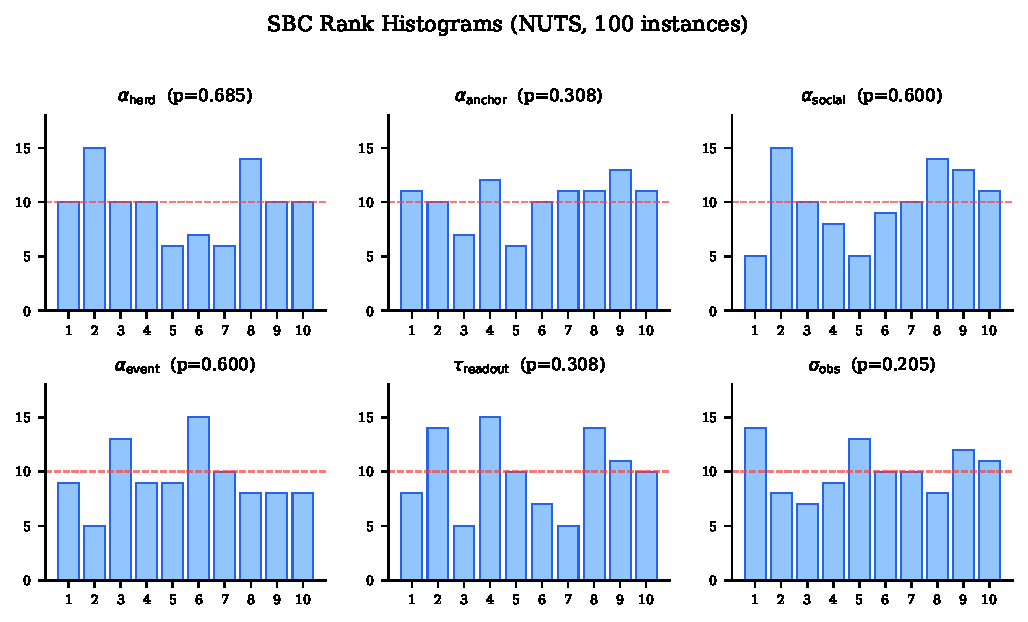
\includegraphics[width=\textwidth]{figures/fig2_sbc.pdf}
    \caption{SBC rank histograms ($2 \times 3$ grid). Each panel shows the rank histogram for one parameter. Horizontal dashed line at expected count $= 10$ (uniform). All histograms appear roughly uniform, confirming well-calibrated posteriors under NUTS.}
    \label{fig:sbc}
\end{figure}

\subsection{Evolution from v1 to \textsc{Base}}

\begin{table}[H]
\centering
\caption{v1 vs \textsc{Base} Comparison}
\label{tab:v1v2}
\begin{adjustbox}{max width=\textwidth}
\begin{tabular}{@{}lll@{}}
\toprule
Aspect & v1 (unpublished prototype) & \textsc{Base} (this paper) \\
\midrule
Calibration & Grid search (972 combos) & Hierarchical Bayesian SVI \\
Training data & 1000 LLM-generated scenarios & 42 empirical scenarios \\
Parameters & 5 (all ad hoc) & 4 calibrable + 4 frozen \\
Uncertainty & None & 90\% CI, coverage 75.0\% ($N{=}8$) \\
Discrepancy & None & Explicit $b_d + b_s$ \\
Validation & Same data as training & Held-out test set + SBC \\
Online assim. & None & EnKF (proof of concept, in-sample) \\
MAE (test) & 14.8~pp (synthetic)* & 19.2~pp (empirical, $N{=}8$)* \\
\bottomrule
\end{tabular}
\end{adjustbox}

\vspace{4pt}
\footnotesize
*Direct comparison is not straightforward: v1 was evaluated on LLM-generated synthetic scenarios while \textsc{Base} uses empirical scenarios with real-world ground truth. The v1 test set likely understates true error because synthetic ground truth inherits the same LLM biases as the simulation (epistemic circularity).
\end{table}

\subsection{Covariate Effects}

Of the 20 entries in the $B$ matrix (4 parameters $\times$ 5 covariates), one effect is statistically significant at the 95\% level. With 34 training scenarios and 20 coefficients, statistical power is limited. No correction for multiple comparisons is applied.

\begin{table}[H]
\centering
\caption{Covariate Effects}
\label{tab:covariates}
\begin{adjustbox}{max width=\textwidth}
\begin{tabular}{@{}lllll@{}}
\toprule
Parameter & Covariate & $B_{ij}$ & 95\% CI & Interpretation \\
\midrule
$\alpha_{\text{event}}$ & inst.\ trust & $-0.127$ & $[-0.242, -0.015]$ & Higher trust reduces event sensitivity \\
\bottomrule
\end{tabular}
\end{adjustbox}
\end{table}

In scenarios with high institutional trust, external shocks are absorbed by institutional credibility rather than amplified through the opinion network. The two nearest-to-significant effects---$\alpha_{\text{anchor}} \times \text{undecided\_share}$ ($B = +0.116$, CI $[-0.010, 0.243]$) and $\alpha_{\text{herd}} \times \text{initial\_polarization}$ ($B = +0.096$, CI $[-0.013, 0.217]$)---are substantively plausible but require a larger dataset to confirm.

\subsection{Calibration Evolution Details}
\label{app:evolution_details}

This subsection provides additional detail for the three calibration variants summarised in Section~\ref{sec:evolution}.

\textbf{\textsc{Ground} (Selective Grounding).} Domains with mean absolute scenario discrepancy $|b_s| > 0.4$ (financial: 0.744, energy: 0.709, public health: 0.534, corporate: 0.432) were grounded by replacing LLM-generated events with Google Search-verified historical events. Domains with low discrepancy (political, technology) were left unchanged, producing 20 grounded + 22 unchanged = 42 total scenarios. The coverage collapse from 79.4\% to 2.9\% occurred because verified events constrained the event force term, reducing the discrepancy budget available to $b_s$ and producing unrealistically tight credible intervals.

\textbf{\textsc{Hybrid} (Hybrid Grounding).} Combined original LLM agents with Google Search-verified events in a hybrid approach on 20 curated high-quality scenarios (15 train / 5 test). The between-domain discrepancy $\sigma_{b,\text{between}}$ increased from 0.115 to 0.358 logit while within-scenario discrepancy remained stable, indicating better separation of domain-level bias from scenario-specific noise. Test-set coverage: 80.0\% (4/5), with AMC Short Squeeze as the sole outlier.

\textbf{\textsc{Poll} (PubOp Agent).} The Public Opinion agent is configured as a citizen with low rigidity (0.1), high tolerance (0.9), high influence (0.7), and cluster size proportional to poll sample size. Its initial position $p_{\text{pubop}} = 2 (\text{pro\_pct}/100) - 1$ acts as a gravity well pulling the citizen swarm toward the empirically observed distribution, correcting systematic LLM bias toward centrist positions. Its low rigidity ensures the anchor drifts naturally with events. Since \textsc{Poll} uses strictly more information than \textsc{Hybrid} (the initial polling observation), the improvement in training coverage (86.7\%) cannot be attributed solely to the agent architecture.

\textbf{Financial outlier analysis.} Across all versions, financial scenarios exhibit the largest errors. Three patterns recur: (i)~trust cascades (binary collapse vs.\ survive dynamics), (ii)~contagion effects that bounded-confidence social influence cannot express, and (iii)~threshold nonlinearity (abrupt phase transitions vs.\ the model's continuous evolution assumption). Domain-specific force functions---potentially incorporating regime switching (Section~\ref{sec:regime})---are needed for financial crisis modeling.

\begin{table}[H]
\centering
\caption{Cross-variant metrics. Differing test sets ($N=8$ vs $N=5$) and information sets (poll-free vs poll-informed) preclude direct ranking. Binomial 95\% CIs on coverage: 75.0\% ($N=8$): [34.9, 96.8]\%; 80.0\% ($N=5$): [28.4, 99.5]\%. $\dagger$Poll-informed.}
\label{tab:versions}
\begin{adjustbox}{max width=\textwidth}
\begin{tabular}{@{}llcccccc@{}}
\toprule
Variant & Strategy & Scenarios & MAE test & MAE train & RMSE test & Cov.\ 90\% (test) & Cov.\ 90\% (train) \\
\midrule
\textsc{Base}    & Discrepancy only      & 42 (34/8) & 19.2~pp & 14.3~pp & 26.6~pp & 75.0\% (6/8) & 79.4\% \\
\textsc{Ground}  & Verified events  & 42 (34/8) & 18.9~pp & 15.1~pp & 21.6~pp & --- & 2.9\% \\
\textsc{Hybrid}  & LLM + verified events & 20 (15/5) & 11.4~pp & 15.3~pp & 16.8~pp & 80.0\% (4/5) & 73.3\% \\
\textsc{Poll}$\dagger$ & Hybrid + poll anchor & 20 (15/5) & 13.6~pp & 13.9~pp & 20.0~pp & 80.0\% (4/5) & 86.7\% \\
\bottomrule
\end{tabular}
\end{adjustbox}
\end{table}

\section{Reproducibility of the v2.5 Benchmark Layer}
\label{app:reproducibility}

All numerical results in Sections~\ref{sec:dm_benchmark}--\ref{sec:matrix} are produced by a self-contained Python module released alongside the codebase. This appendix documents the package, its command-line interface, and its automated test suite so that the reference distribution can be rederived from scratch and any modification to the sim can be re-evaluated against it.

\subsection{Module Layout}
\label{app:repro_layout}

The \texttt{benchmarks/} package contains six first-class modules:

\begin{table}[H]
\centering
\caption{Module layout of the \texttt{benchmarks/} package.}
\label{tab:repro_modules}
\begin{adjustbox}{max width=\textwidth}
\begin{tabular}{@{}p{4cm}p{12cm}@{}}
\toprule
File & Responsibility \\
\midrule
\texttt{forecasters.py} & Closed-form null baselines: naive persistence, running mean, OLS linear trend, AR(1). Exposes \texttt{generate\_baseline\_trajectory} for one-step-ahead rolling forecasts and \texttt{forecast\_errors}~/ \texttt{rmse} helpers. \\
\texttt{diebold\_mariano.py} & DM statistic with the Harvey--Leybourne--Newbold correction. Student-$t$ p-values computed via the regularized incomplete beta identity $P(T > x) = \tfrac{1}{2} I_{\nu/(\nu+x^2)}(\nu/2, 1/2)$ with Lentz's continued-fraction expansion --- no SciPy dependency. \\
\texttt{coverage.py} & Empirical coverage of an interval sequence against realized values, plus a nonparametric bootstrap confidence band on the coverage statistic itself. Includes a \texttt{coverage\_from\_quantiles} helper for ensemble Monte Carlo intervals. \\
\texttt{residual\_ci.py} & Residual-bootstrap predictive intervals that turn any point-forecaster into a calibrated interval forecaster, enabling the model-free coverage check of Section~\ref{sec:residual_cov}. \\
\texttt{scenario\_matrix.py} & Enumeration of the $7 \times 5 \times 4$ scenario-diversity axis, \texttt{ScenarioCell} dataclass, and a \texttt{coverage\_report} that flags missing axis values in any given corpus. \\
\texttt{historical.py}~/ \texttt{historical\_runner.py} & Loader that normalizes the v1 and v2.2 empirical JSON scenarios into the common \texttt{support}~/ \texttt{signed\_position} representation, derives tension from per-scenario volatility, maps ISO country codes to regions, and runs all baselines + DM tests + coverage + matrix report in one pass. \\
\texttt{runner.py} & Parallel runner for the deterministic-trajectory benchmark against the 7 scenarios stored in \texttt{frontend/public/data/scenario\_*} (the sim-forecast case). \\
\bottomrule
\end{tabular}
\end{adjustbox}
\end{table}

\subsection{Command-Line Usage}
\label{app:repro_cli}

The historical benchmark (Sections~\ref{sec:dm_benchmark}--\ref{sec:matrix}) regenerates from scratch with:

\begin{verbatim}
python -m benchmarks.historical_runner \
    --out outputs/historical_benchmark.json \
    --markdown outputs/historical_benchmark.md
\end{verbatim}

The deterministic-trajectory benchmark (sim-forecast case, for continuous regression testing) runs with:

\begin{verbatim}
python -m benchmarks \
    --out outputs/benchmark_report.json \
    --markdown outputs/benchmark_report.md
\end{verbatim}

Both commands are zero-configuration on the public repository and write machine-readable JSON + human-readable Markdown reports.

\subsection{Automated Test Suite}
\label{app:repro_tests}

The benchmark layer ships with 103 automated tests distributed across five files and four markers (\texttt{slow}, \texttt{integration}, \texttt{perf}, \texttt{stress}):

\begin{table}[H]
\centering
\caption{Test-suite composition for the v2.5 benchmark layer.}
\label{tab:repro_tests}
\begin{adjustbox}{max width=\textwidth}
\begin{tabular}{@{}p{5.5cm}cp{9cm}@{}}
\toprule
Test file & Tests & Purpose \\
\midrule
\texttt{test\_benchmarks.py} & 18 & Unit tests for forecasters, DM, coverage, scenario matrix. \\
\texttt{test\_benchmarks\_integration.py} &  8 & End-to-end runner tests, including residual-bootstrap calibration on i.i.d.\ noise. \\
\texttt{test\_performance\_sla.py} &  5 & Throughput SLAs for DM, coverage, baselines, and the runner (defaults: 1000 DM tests in $<$~5~s, runner on 20 synthetic scenarios in $<$~3~s). All thresholds env-overridable via \texttt{DTS\_SLA\_*}. \\
\texttt{test\_stress\_scenarios.py} & 57 & Adversarial-signal stress tests (flat, monotone, alternating, spike, heavy-tail, near-constant), DM sign-consistency under $a \leftrightarrow b$ swap, coverage boundedness under random intervals, per-cell smoke tests on the full scenario matrix. \\
\texttt{test\_historical\_benchmark.py} & 15 & Unit + integration tests for the empirical loader (including v1/v2.2 duplicate resolution, \texttt{None}-field tolerance, and domain-alias collapse) and the aggregate runner. Includes a corpus smoke test that fails loudly if the matrix coverage regresses. \\
\bottomrule
\end{tabular}
\end{adjustbox}
\end{table}

Total runtime on a laptop-class machine: 2.94 seconds for the full 103-test suite, which is kept under 5 seconds so it can run on every commit without gating.

\subsection{Release Artifacts}
\label{app:repro_artifacts}

Running the two commands above produces four reproducible artifacts shipped with the paper:

\begin{enumerate}
    \item \texttt{outputs/historical\_benchmark.json} --- the full per-scenario $\times$ per-metric $\times$ per-baseline score matrix ($43 \times 2 \times 4 = 344$ score rows).
    \item \texttt{outputs/historical\_benchmark.md} --- the human-readable summary from which Tables~\ref{tab:dm_support}, \ref{tab:dm_signed}, \ref{tab:dm_by_domain}, and~\ref{tab:matrix_cov} are extracted verbatim.
    \item \texttt{outputs/benchmark\_report.json} --- the deterministic-trajectory benchmark on the 7 scenarios currently shipped with the frontend, used as a continuous regression signal.
    \item \texttt{outputs/benchmark\_report.md} --- the corresponding Markdown summary.
\end{enumerate}

Any future modification to the simulator, the calibration pipeline, or the EnKF can be A/B-tested against the v2.5 reference distribution by running the two commands before and after the change. Disagreement on any DM cell at $p < 0.05$ constitutes a reproducibility-relevant regression.

\begin{thebibliography}{99}

\bibitem[Argyle et~al.(2023)]{argyle2023}
Argyle, L.~P., Busby, E.~C., Fulda, N., Gubler, J.~R., Rytting, C., \& Wingate, D. (2023).
\newblock Out of one, many: Using language models to simulate human samples.
\newblock \textit{Political Analysis}, 31(3), 337--351.

\bibitem[Blei et~al.(2017)]{blei2017}
Blei, D.~M., Kucukelbir, A., \& McAuliffe, J.~D. (2017).
\newblock Variational inference: A review for statisticians.
\newblock \textit{Journal of the American Statistical Association}, 112(518), 859--877.

\bibitem[Festinger(1957)]{festinger1957}
Festinger, L. (1957).
\newblock \textit{A Theory of Cognitive Dissonance}.
\newblock Stanford University Press.

\bibitem[Deffuant et~al.(2000)]{deffuant2000}
Deffuant, G., Neau, D., Amblard, F., \& Weisbuch, G. (2000).
\newblock Mixing beliefs among interacting agents.
\newblock \textit{Advances in Complex Systems}, 3(01n04), 87--98.

\bibitem[DeGroot(1974)]{degroot1974}
DeGroot, M.~H. (1974).
\newblock Reaching a consensus.
\newblock \textit{Journal of the American Statistical Association}, 69(345), 118--121.

\bibitem[Diebold \& Mariano(1995)]{diebold1995}
Diebold, F.~X., \& Mariano, R.~S. (1995).
\newblock Comparing predictive accuracy.
\newblock \textit{Journal of Business \& Economic Statistics}, 13(3), 253--263.

\bibitem[Flache et~al.(2017)]{flache2017}
Flache, A., M\"as, M., Feliciani, T., Chattoe-Brown, E., Defuant, G., Huet, S., \& Lorenz, J. (2017).
\newblock Models of social influence: Towards the next frontiers.
\newblock \textit{Journal of Artificial Societies and Social Simulation}, 20(4), 2.

\bibitem[Evensen(2003)]{evensen2003}
Evensen, G. (2003).
\newblock The Ensemble Kalman Filter: Theoretical formulation and practical implementation.
\newblock \textit{Ocean Dynamics}, 53(4), 343--367.

\bibitem[Gao et~al.(2024)]{gao2023}
Gao, C., Lan, X., Li, N., Yuan, Y., Ding, J., Zhou, Z., \ldots\ \& Li, Y. (2024).
\newblock Large language models empowered agent-based modeling and simulation: A survey and perspectives.
\newblock \textit{Humanities and Social Sciences Communications}, 11, 1--15.

\bibitem[Grimm et~al.(2006)]{grimm2006}
Grimm, V., Berger, U., Bastiansen, F., Eliassen, S., Ginot, V., Giske, J., \ldots\ \& DeAngelis, D.~L. (2006).
\newblock A standard protocol for describing individual-based and agent-based models.
\newblock \textit{Ecological Modelling}, 198(1--2), 115--126.

\bibitem[Grimm et~al.(2010)]{grimm2010}
Grimm, V., Berger, U., DeAngelis, D.~L., Polhill, J.~G., Giske, J., \& Railsback, S.~F. (2010).
\newblock The ODD protocol: A review and first update.
\newblock \textit{Ecological Modelling}, 221(23), 2760--2768.

\bibitem[Grazzini et~al.(2017)]{grazzini2017}
Grazzini, J., Richiardi, M.~G., \& Tsionas, M. (2017).
\newblock Bayesian estimation of agent-based models.
\newblock \textit{Journal of Economic Dynamics and Control}, 77, 26--47.

\bibitem[Harvey et~al.(1997)]{harvey1997}
Harvey, D., Leybourne, S., \& Newbold, P. (1997).
\newblock Testing the equality of prediction mean squared errors.
\newblock \textit{International Journal of Forecasting}, 13(2), 281--291.

\bibitem[Hegselmann \& Krause(2002)]{hegselmann2002}
Hegselmann, R., \& Krause, U. (2002).
\newblock Opinion dynamics and bounded confidence: models, analysis and simulation.
\newblock \textit{Journal of Artificial Societies and Social Simulation}, 5(3).

\bibitem[Holley \& Liggett(1975)]{holley1975}
Holley, R.~A., \& Liggett, T.~M. (1975).
\newblock Ergodic theorems for weakly interacting infinite systems and the voter model.
\newblock \textit{The Annals of Probability}, 3(4), 643--663.

\bibitem[Horton et~al.(2024)]{horton2023}
Horton, J.~J., Filippas, A., \& Manning, R. (2024).
\newblock Large language models as simulated economic agents: What can we learn from homo silicus?
\newblock In \textit{Proceedings of the 25th ACM Conference on Economics and Computation (EC '24)}.

\bibitem[Kennedy \& O'Hagan(2001)]{kennedy2001}
Kennedy, M.~C., \& O'Hagan, A. (2001).
\newblock Bayesian calibration of computer models.
\newblock \textit{Journal of the Royal Statistical Society: Series B}, 63(3), 425--464.

\bibitem[Mistry et~al.(2021)]{mistry2021}
Mistry, D., Litvinova, M., Chinazzi, M., et~al. (2021).
\newblock Inferring high-resolution human mixing patterns for disease modeling.
\newblock \textit{Nature Communications}, 12(1), 323.

\bibitem[Park et~al.(2023)]{park2023}
Park, J.~S., O'Brien, J.~C., Cai, C.~J., Morris, M.~R., Liang, P., \& Bernstein, M.~S. (2023).
\newblock Generative agents: Interactive simulacra of human behavior.
\newblock In \textit{Proceedings of the 36th Annual ACM Symposium on User Interface Software and Technology}.

\bibitem[Park et~al.(2022)]{park2022}
Park, J.~S., Popowski, L., Cai, C., Morris, M.~R., Liang, P., \& Bernstein, M.~S. (2022).
\newblock Social simulacra: Creating populated prototypes for social computing systems.
\newblock In \textit{Proceedings of the 35th Annual ACM Symposium on User Interface Software and Technology}.

\bibitem[Platt(2020)]{platt2020}
Platt, D. (2020).
\newblock A comparison of economic agent-based model calibration methods.
\newblock \textit{Journal of Economic Dynamics and Control}, 113, 103859.

\bibitem[Reich \& Cotter(2015)]{reich2015}
Reich, S., \& Cotter, C. (2015).
\newblock \textit{Probabilistic Forecasting and Bayesian Data Assimilation}.
\newblock Cambridge University Press.

\bibitem[Saltelli et~al.(2008)]{saltelli2008}
Saltelli, A., Ratto, M., Andres, T., Campolongo, F., Cariboni, J., Gatelli, D., \ldots\ \& Tarantola, S. (2008).
\newblock \textit{Global Sensitivity Analysis: The Primer}.
\newblock John Wiley \& Sons.

\bibitem[Sobol(2001)]{sobol2001}
Sobol, I.~M. (2001).
\newblock Global sensitivity indices for nonlinear mathematical models and their Monte Carlo estimates.
\newblock \textit{Mathematics and Computers in Simulation}, 55(1--3), 271--280.

\bibitem[Talts et~al.(2018)]{talts2018}
Talts, S., Betancourt, M., Simpson, D., Vehtari, A., \& Gelman, A. (2018).
\newblock Validating Bayesian inference algorithms with simulation-based calibration.
\newblock \textit{arXiv preprint arXiv:1804.06788}.

\bibitem[Thiele et~al.(2014)]{thiele2014}
Thiele, J.~C., Kurth, W., \& Grimm, V. (2014).
\newblock Facilitating parameter estimation and sensitivity analysis of agent-based models: A cookbook using NetLogo and R.
\newblock \textit{Journal of Artificial Societies and Social Simulation}, 17(3), 11.

\bibitem[Windrum et~al.(2007)]{windrum2007}
Windrum, P., Fagiolo, G., \& Moneta, A. (2007).
\newblock Empirical validation of agent-based models: Alternatives and prospects.
\newblock \textit{Journal of Artificial Societies and Social Simulation}, 10(2), 8.

\end{thebibliography}

\end{document}
